\documentclass[10pt]{article}
\usepackage[utf8]{inputenc}
\usepackage{empheq}
\usepackage[inline, shortlabels]{enumitem}
\usepackage{gensymb}
\usepackage{multicol}
\setlength{\parskip}{0.5cm plus4mm minus3mm}
\setlength{\parindent}{0pt}
\usepackage{amsmath}
\usepackage{upgreek}
\usepackage[nobreak=true]{mdframed}
\usepackage[margin=0.6in]{geometry}
 \geometry{
 left=12mm,
 bottom=20mm
 }
\usepackage{amssymb}
\usepackage{cs170}
\usepackage{titlesec}
\usepackage{comment}
\usepackage{chngcntr}
\usepackage{graphicx}
\usepackage{booktabs}
\usepackage{changepage}
\usepackage{chngcntr}
\usepackage{scrextend}
\usepackage{adjustbox}

\newcommand*{\horzbar}{\rule[.5ex]{2.5ex}{0.5pt}}

\begin{document}
\date{}
\author{}
\title{\vspace{-5ex} \dunhd{CS189: Machine Learning Notes} \vspace{-5ex}}
\maketitle

%%%%%%%%%%%%%%%%%%%%%%%%%%%%%%%%%%%%%%%%%%
%      COMMENT ABOUT THE NOTES           %
%%%%%%%%%%%%%%%%%%%%%%%%%%%%%%%%%%%%%%%%%%
\begin{comment}
It is recommended (but not necessary) to take CS170 or CS188 before CS189. The first two sections of CS188 (Search & Planning, Probabilistic Inference) provide useful background knowledge for ML. The last section of CS188 can be safely ignored, as this class covers ML in far greater detail.

A mathematical foundation in multivariable calculus, linear algebra, and probability is assumed. An appendix of the topics in each field most relevant to machine learning is included at the end. 

These notes serve as an introduction to the field of machine learning, and are not at all comprehensive. We are primarily concerned with the main ideas behind core ML techniques. Notably, we omit reinforcement learning completely (however, RL is covered fairly well in CS188).

Also note that we aren't concerned with the implementation of any of the algorithms. We rest assured that there exist ML libraries that implement all of the techniques to be discussed efficiently.
\end{comment}

\begin{multicols}{2}
\section{Linear Regression}
\vspace{-0.2cm}
\begin{addmargin}[0.8em]{0.5em}
    \subsection{Introduction}
    \vspace{-0.2cm}
    \begin{enumerate}[label=(\alph*)]
        \item Machine learning explores the study and construction of algorithms that can learn from and make predictions on data.
        \item Levels of abstraction in ML:
        \begin{enumerate}
            \item \textit{Applications and Data}: identify the problem and the nature of the data.
            \item \textit{Model}: choose the mathematical model that best represents the pattern we wish to learn.
            \item \textit{Optimization Problem}: cast the problem of finding the right model into a concrete optimization problem (e.g. minimize an objective function).
            \item \textit{Optimization Algorithm}: determine how to solve the optimization problem.
        \end{enumerate}
    \end{enumerate}  
    \vspace{-0.2cm}
    \subsection{Ordinary Least Squares}
    \vspace{-0.2cm}
    \begin{enumerate}[label=(\alph*)]
        \item In statistical modeling, \textit{regression} is the statistical process for estimating the relationships among variables. Ordinary least squares is the simplest technique to solve \textit{linear} regression problems.
        \item The typical set up is as follows: given $n$ $d$-dimensional training samples, we form a matrix $X \in \mathbb{R}^{n \times d}$, and output vector $y \in \mathbb{R}^{n}$. We then solve for the weights $w \in \mathbb{R}^d$:
        \begin{align*}
        w = \arg\min_{w} \| y - X w \|_2^2
        \end{align*}
        A closed form solution is given by
        $$
        w = (X^\top X)^{-1} X^\top y
        $$
        \item Note that OLS can also fit parameters to nonlinear models (e.g. ellipses and cubic functions). We do this by augmenting (in addition to the raw features) new arbitrary features to the data so that the resulting models are still linear with respect to the augmented features.
        
        \item Polynomials are an important class of features. By Taylor’ Theorem, any sufficiently smooth function can be approximated arbitrarily closely by a high enough degree (univariate or multivariate) polynomial. A downside is that a polynomial of degree at most $d$ in $l$ dimensional space has $O(l^d)$ terms.
    
        \item \textbf{Training error} is the prediction error when the model is evaluated on the training data, whereas \textbf{true error} is the prediction error when the model is evaluated on unseen data that comes from the true underlying model. 
        \item Polynomial features in linear regression illustrate this distinction; using higher degree polynomial approximations can lead to reduced training error but increased true error. This is a form of \textbf{overfitting}; the model is too complex, and is fitting the noise. 
    \end{enumerate}
    
    \subsection{Ridge Regression}
    \begin{enumerate}[label=(\alph*)]
        \item OLS becomes numerically unstable when the features of the data are close to collinear. Using the SVD of the feature matrix $A=U\Sigma V^\top$, we find $(A^\top A)^{-1} = V\Sigma^{-2}V^\top$. This shows the singular values of $(A^\top A)^{-1}$ are the squared inverse of the singular values of $A$, which results in extremely large singular values when the singular values of $A$ are near zero.
        \item Ridge regression aims to resolve the numerical instability and overfitting problems of OLS by penalizing the norm of $w$. Precisely, ridge regression is given by the optimization problem
        \begin{align*}
        w = \arg\min_{w} \| y - X w \|_2^2 + \lambda \| w \|_2^2
        \end{align*}
        As with least squares, we can find a closed-form solution to this problem:
        \begin{align*}
        w &= \arg\min_{w} \| y - X w \|_2^2 + \lambda \|w\|_2^2 \\
        &= \arg\min_{w} (y - X w)^\top(y - X w) + \lambda w^\top w \\
        &= \arg\min_{w} y^\top y - 2y^\top X w + w^\top X^\top X w + \lambda w^\top w
        \end{align*}
        We minimize by taking the first derivative and setting it equal to 0:
        \begin{align*}
            \frac{\partial}{\partial w} \left[ y^\top y - 2y^\top X w + w^T X^\top X w + \lambda w^\top w \right] &= 0 \\
            -2X^\top y + 2X^\top X w + 2\lambda w &= 0 \\
            X^\top Xw + \lambda w &= X^\top y \\
            (X^\top X + \lambda I) w &= \lambda y 
        \end{align*}
        So that $w = (X^\top X + \lambda I)^{-1} X^\top y$.
        \item Denoting the singular values of $A$ as $\sigma_i$, the singular values of $(A^\top A + \lambda I)^{-1}$ become $1/(\sigma_i^2 + \lambda^2)$. The initution is that we penalize the weights corresponding to complex features that only serve to fine tune the model and fit noise in the data.
    \end{enumerate}
    
    \subsection{Validation}
    \vspace{-0.2cm}
    \begin{enumerate}[label=(\alph*)]
        \item Hyperparameters are parameters whose values are set prior to the learning process. A \textbf{model hyperparameter} determines the structure of the model (e.g. degree of a polynomial) while an \textbf{optimization hyperparameter} is aspect of the optimization procedure (e.g. choice of $\lambda$ in ridge regression).
        \item A general regression problem attempts to learn a mapping $f: \mathbb{R}^d \mapsto \mathbb{R}$ from samples $\{(x_i, y_i)\}_{i=1}^n$, where $y_i \approx f(x_i)$. That is, we find weights $\alpha$ where
        $$
        f_\alpha(x) = \sum_{j=1}^p \alpha_j \underbrace{\phi(x)}_{\text{features}}
        $$
        Define the \textbf{mean squared error} as
        $$
        \frac{1}{n} \sum_{i=1}^n (f_\alpha(x_i) - y_i)^2
        $$
        and the true error as
        $$
        \mathbb{E} \left[ (f_\alpha(x) - y)^2 \right]
        $$
        We cannot compute the true error, but we can estimate it with validation data.
        \item The idea is to partition the training data into a \textit{training set}, \textit{validation set}, and \textit{test set}. A simple way to choose hyperparameters, then, is to choose the configuration with the lowest validation error. Test error should be used to compare results between different models or algorithms.
        \item Cross-validation is an alternative to having a dedicated validation set. $k$-fold cross-validation works as follows:
        \begin{enumerate}
        \item Shuffle the data and partition it into $k$ blocks.
        \item For $i=1$ to $k$, train the model on all blocks except $i$ and compute the validation error on block $i$.
        \item Average the $k$ validation errors to obtain an estimate of the true error.
        \end{enumerate}
    \end{enumerate}
    
    \vspace{-0.2cm}
    \subsection{Probabilistic Interpretations}
    \vspace{-0.2cm}
    \begin{enumerate}[label=(\alph*)]
        \item Now we use statistical interpretations of regression methods to see what we’ve done so far through a different perspective.
        \item Consider the data samples we observe as random variables with specific distributions (e.g. uniform, normal, Laplacian). We focus on Gaussians, as random noise is often assumed to be normally distributed.
        \item Suppose we assume our observations are noisy, i.e. $y_i = f(x_i) + N_i$ where $f$ is the true underlying model and $N_i$ is a random variable. If we assume $N_i \sim \mathcal{N}(0, \sigma^2)$, then $y_i \mid x_i \sim \mathcal{N}(f(x_i), \sigma^2)$.
        
        \item We can use MLE to solve for the model $h$ that maximizes the probability of the data. Going straight to the log-likelihood, we have
        \begin{align*}
        h^{*}_{\text{MLE}} &= \arg\max_{h} \sum_{i=1}^{n} \log{P(y_i \mid x_i, h)} \\
        &= \arg\max_{h} - \left( \sum_{i=1}^{n} \frac{(y_i - h(x_i))^2}{2\sigma^2} \right) - n\log{\sqrt{2\pi}\sigma} \\
        &= \arg\min_{h} \left( \sum_{i=1}^{n} \frac{(y_i - h(x_i))^2}{2\sigma^2} \right) + n\log{\sqrt{2\pi}\sigma} \\
        &= \arg\min_{h}  \sum_{i=1}^{n} (y_i - h(x_i))^2       
        \end{align*}
        Taking $h$ as some linear combination of features of $x$, this is exactly the OLS setup. Thus, OLS is the solution to MLE under a Gaussian noise model.
        \item If we apply MAP to the same setup, now we assume $h$ has a \textit{prior} $P(h)$ such that $h \sim \mathcal{N}(h_0, \sigma^2_h I)$. Going straight to the log-likelihood, we have
        \begin{align*}
        h^*_{\text{MAP}} &= \arg\max_{h} \left( \log{P(h)} + \sum_{i=1}^n \log{P(y_i | x_i, h)} \right) \\
        &= \arg\max_{h} - \frac{\sum_{i=1}^{n} (y_i - h(x_i))^2)}{2\sigma^2} - \frac{\| h - h_0 \|_2^2}{2\sigma_h^2}  \\
        &= \arg\min_{h}   \frac{\sum_{i=1}^{n} (y_i - h(x_i))^2)}{2\sigma^2} +  \frac{\| h - h_0 \|_2^2}{2\sigma_h^2}  \\
        &= \arg\min_{h} \sum_{i=1}^{n} (y_i - h(x_i))^2  + \frac{\sigma^2}{\sigma_h^2}  \| h - h_0 \|_2^2
        \end{align*}
        Taking $\lambda = \frac{\sigma^2}{\sigma_h^2}$, this is exactly the ridge regression setup. Thus, MAP is a probabilistic justification for adding the penalized term in ridge regression. 
        
        \item For small data sets, MAP can produce a better or worse solution than MLE, depending on the quality of the prior. With enough data, the prior term becomes irrelevant.
    \end{enumerate}    

    \subsection{Bias-Variance Tradeoff}
    \begin{enumerate}[label=(\alph*)]
        \item Now we form a theoretical metric to better understand the phenomena of overfitting. 
        \item Mathematically, we represent the metric as the expected squared error between the hypothesis $h$ and the observation $Y = f(x) + N$:
        $$
        \epsilon(x;h) = \mathbb{E} \left[ (h(x;D) - Y)^2 \right]
        $$
        where here we treat the $x$'s as fixed constants and the data set $D$ and $Y$ as independent random variables. Note that
        \begin{align*}
        \mathbb{E}[Y] &= \mathbb{E} \left[ f(x) + N \right] = f(x) + \mathbb{E} \left[ N \right] = f(x) \\
        \text{Var}(Y) &= \text{Var}(f(x) + N) = \text{Var}(N)
        \end{align*}
        \item Decomposing the error metric, we have
        \begin{align*}
        &\epsilon(x;h) \\
        &= \mathbb{E} \left[ (h(x;D) - Y)^2 \right] \\
        &= \mathbb{E} \left[ (h(x;D))^2 \right] + \mathbb{E} \left[ Y^2 \right] -2 \mathbb{E} \left[ h(x;D) \cdot Y) \right] \\
        &= \left( \text{Var}(h(x;D)) + \mathbb{E} \left[ h(x;D) \right]^2 \right) \\
        &+ \left( \text{Var}(Y) + \mathbb{E}[Y]^2 \right) -2 \mathbb{E} \left[ h(x;D) \right] \cdot \mathbb{E}[Y] \\
        &= \left( \mathbb{E} \left[ h(x;D) \right]^2 - 2 \mathbb{E}[h(x;D)] \cdot \mathbb{E}[Y] + \mathbb{E}[Y]^2 \right) \\
        &+ \text{Var}(h(x;D)) + \text{Var}(Y) \\
        &= \left( \mathbb{E} \left[ h(x;D) \right] - \mathbb{E}[Y] \right)^2 + \text{Var}(h(x;D)) + \text{Var}(Y) \\
        &= \left( \mathbb{E} \left[ h(x;D) \right] - f(x) \right)^2 + \text{Var}(h(x;D)) + \text{Var}(N)
        \end{align*}
        The second line follows from $\mathbb{E}[X^2] = \text{Var}(X)+ \mathbb{E}[X]^2$ for any r.v. $X$. Also, if $X$ and $Y$ are independent, then so are $g_1(X)$ and $g_2(Y)$ for any functions $g_1$, $g_2$. Hence $h(x;D)$ and $Y$ are independent.
        \item The final decomposition is called the bias-variance decomposition. The first term is the square of the \textit{bias} of the method. The second term is the \textit{variance} of the method. The last term is the \textit{irreducible error}.
        \item Underfitting is equivalent to high bias; overfitting correlates to high variance. Training error reflects bias but not variance, while test error reflects both. 
        \item Adding good features will decrease the bias, but adding a bad feature will rarely increase the bias. However, adding a feature usually increases the variance, so a feature should only be added if it decreases bias more than it increases variance.
    \end{enumerate}
    
    \subsection{Weighted Least Squares}
    \begin{enumerate}[label=(\alph*)]
        \item We now consider regression with non-identically distributed noise, and later, with dependent noise. From this point forward it becomes easier to reason from the probabilistic perspective.
        \item We first approach weighted least squares from an optimization perspective. The idea is to weight certain data points more than others:
        \begin{align*}
        w = \arg\min_{w} \sum_{i=1}^{n} \omega_i (y_i - \phi(x_i)^\top w)^2
        \end{align*}
        i.e., the same as OLS except each data point is weighted by $\omega_i$. In vector form,
        \begin{align*}
        w = \arg\min_{w} (y - Xw)^\top \Omega (y - Xw)
        \end{align*}
        where the $i$-th row of $X$ is $\phi(x_i)^\top$ and $\Omega = \text{diag}(\omega_1, \hdots, \omega_n)$. We expand this out to see an identical formulation to OLS, except the feature matrix and observation matrix are scaled by $\Omega^{1/2}$. The solution is then
        \begin{align*}
        w = (X^\top \Omega X)^{-1} X^\top \Omega y
        \end{align*}
        \item Now we take a probabilistic approach via MLE. Our model is
        \begin{align*}
        y_i = \phi(x_i)^\top w + Z_i
        \end{align*}
        where the $Z_i$ are independent Gaussians, but \textit{not} identically distributed: $Z_i \sim \mathcal{N}(0, \sigma_i^2)$. We can make the $Z_i$'s i.i.d. by scaling the data:
        \begin{align*}
        \frac{y_i}{\sigma_i} = \frac{\phi(x_i)^\top w}{\sigma_i} + \frac{Z_i}{\sigma_i}
        \end{align*}
        The MLE is then given by
        \begin{align*}
        \arg\min_{w} \left( \sum_{i=1}^{n} \frac{(\frac{y_i}{\sigma_i} - \frac{\phi(x_i)^\top w}{\sigma_i})^2}{2} \right) + n\log{\sqrt{2\pi}}
        \end{align*}
        This scaled MLE problem has the same setup as that above, so that the solution is
        \begin{align*}
        w = (X^\top \Sigma_Z^{-1} X)^{-1} X^\top \Sigma_Z^{-1} y
        \end{align*}
        where 
        $$
        \Sigma_Z =
        \left[
        \begin{array}{cccc} 
        \sigma^{2}_{1} & 0 &   \ldots & 0 \\ 0 & \sigma^{2}_{2} & \ldots & 0 \\  \vdots  & \vdots & \ddots & \vdots \\ 0 & 0 & \ldots  &  \sigma^{2}_{n}
        \end{array} 
        \right]
        $$
        Hence the probabilistic perspective sets $\omega_i = \frac{1}{\sigma_i^2}$. Intuitively, as the variance of the noise increases, we ``trust" that data point less.
        
        \item We have assumed the $Z_i$'s are independent. If not (i.e., there is \textit{colored} noise) we can always represent the noise vector $\mathbf{Z}$ as
        $$
        \mathbf{Z} = R \mathbf{U} + \mu
        $$
        for some $R\in \mathbb{R}^{n\times n}$ and $\mu \in \mathbb{R}^n$ where $\mathbf{Z}, \mathbf{U} \in \mathbb{R}^n$ are random vectors and each $U_i \sim \mathcal{N}(0,1)$ is i.i.d.. In this case, $\mathbf{Z} \sim \mathcal{N}(\mu, \Sigma_Z)$ where $\Sigma_Z= RR^\top$. 
        \item In the case $\mu=\vec{0}$, for example, we have $y=Xw+\mathbf{Z}$ as before, except now $\mathbf{Z}$ is jointly Gaussian so that $y \sim \mathcal{N}(Xw, \Sigma_Z)$. We reduce this back into an MLE problem with i.i.d noise by premultiplying $X$ and $y$ by $\Sigma_Z^{-1/2}$. The solution is as in the independent case:
        \begin{align*}
        w = (X^\top \Sigma_Z^{-1} X)^{-1} X^\top \Sigma_Z^{-1} y
        \end{align*}        
    \end{enumerate}
    
    \subsection{MAP with colored noise}
    \begin{enumerate}[label=(\alph*)]
        \item Now we see how MAP deals with colored noise. In deriving ridge regression via MAP, our prior assumed that $w_i$ were i.i.d. univariate Gaussians. Now we allow $w \sim \mathcal{N}(\mu_w, \Sigma_w)$, i.e., any multivariate Gaussian. We can rewrite any multivariate Gaussian as an affine transformation of a standard Gaussian:
        $$
        w = \Sigma_w^{1/2} v + \mu_w
        $$
        where $v \sim \mathcal{N}(0, I)$. Plugging this reparameterization into the approximation $y \approx Xw$ gives
        $$
        X \Sigma_w^{1/2} v \approx y - X \mu_w
        $$
        Applying MAP (i.e. ridge regression) as before with these new coordinates gives
        $$
        v = (\Sigma_w^{\frac{\top}{2}} X^\top X \Sigma_w^{\frac{1}{2}} + I)^{-1} \Sigma_w^{\frac{\top}{2}} X^\top (y - X\mu_w)
        $$
        Here we assume the variance of the data is normalized, so that $\lambda=1$. Converting back to $w$, we have
        \begin{align*}
        w &= \mu_w + \Sigma_w^{\frac{1}{2}} (\Sigma_w^{\frac{\top}{2}} X^\top X \Sigma_w^{\frac{1}{2}} + I)^{-1} \Sigma_w^{\frac{\top}{2}} X^\top (y - X\mu_w) \\
        &= \mu_w + (X^\top X + \Sigma_w^{-1})^{-1} X^\top (y - X\mu_w)
        \end{align*}
    \end{enumerate}    
    \vspace{-0.2cm}
    \subsection{Total Least Squares}
    \vspace{-0.2cm}
    \begin{enumerate}[label=(\alph*)]
        \item Total least squares (TLS) arises when measurements of both $x$ and $y$ contain noise. Geometrically, OLS minimizizes the vertical distance between the fitted model and data points, while TLS minimizes the perpendicular distance.
        \item Attempting to differentiate the log-likelihood does not produce a solution. Instead, we develop another formulation that can be solved using the singular value decomposition.
        
        \item \textit{Eckart-Young Theorem}: Consider a matrix $A \in \mathbb{R}^{n \times d}$ with SVD $A = U \Sigma V^\top = \sum_{i=1}^d \sigma_i u_i v_i^\top$. Then
        $$
        A_k = \sum_{i=1}^{k} \sigma_i u_i v_i^\top
        $$
        is the closest rank $k$ matrix to $A$ in  the Frobenius norm.
        
        \item In the 1-dimensional case, our model is
        $$
        (x+\vec{e})w = y + \vec{f}
        $$
        where $\vec{e}$ and $\vec{f}$ are noise vectors for $\vec{x}$ and $\vec{y}$, respectively. We seek $w$ that minimizes the Frobenius norm of the augmented error matrix of $\vec{e}$ and $\vec{f}$.
        \item Through some algebra, we arrive at
        $$
        w = (X^\top X - \sigma_2^2 I)^{-1} X^\top y
        $$
        \item In the general case, if the SVD of $\begin{bmatrix} X & Y \end{bmatrix}$ is
        \begin{align*}
        \begin{bmatrix} X & Y \end{bmatrix} = \begin{bmatrix} U_X & U_Y \end{bmatrix} \begin{bmatrix} \Sigma_X & 0 \\ 0 & \Sigma_Y \end{bmatrix} \begin{bmatrix} V_{XX} & V_{XY} \\ V_{YX} & V_{YY} \end{bmatrix}^\top
        \end{align*}
        then 
        $$
        w = -V_{XY}V_{YY}^{-1}
        $$
    \end{enumerate}
    
    \subsection{Principal Component Analysis}
    \begin{enumerate}[label=(\alph*)]
        \item Principal Component Analysis (PCA) is an unsupervised dimensionality reduction technique. Given a matrix of data points, it finds one or more orthogonal directions that capture the largest amount of variance in the data. It is sensitive to the relative scaling of the original variables.
        \begin{center}
            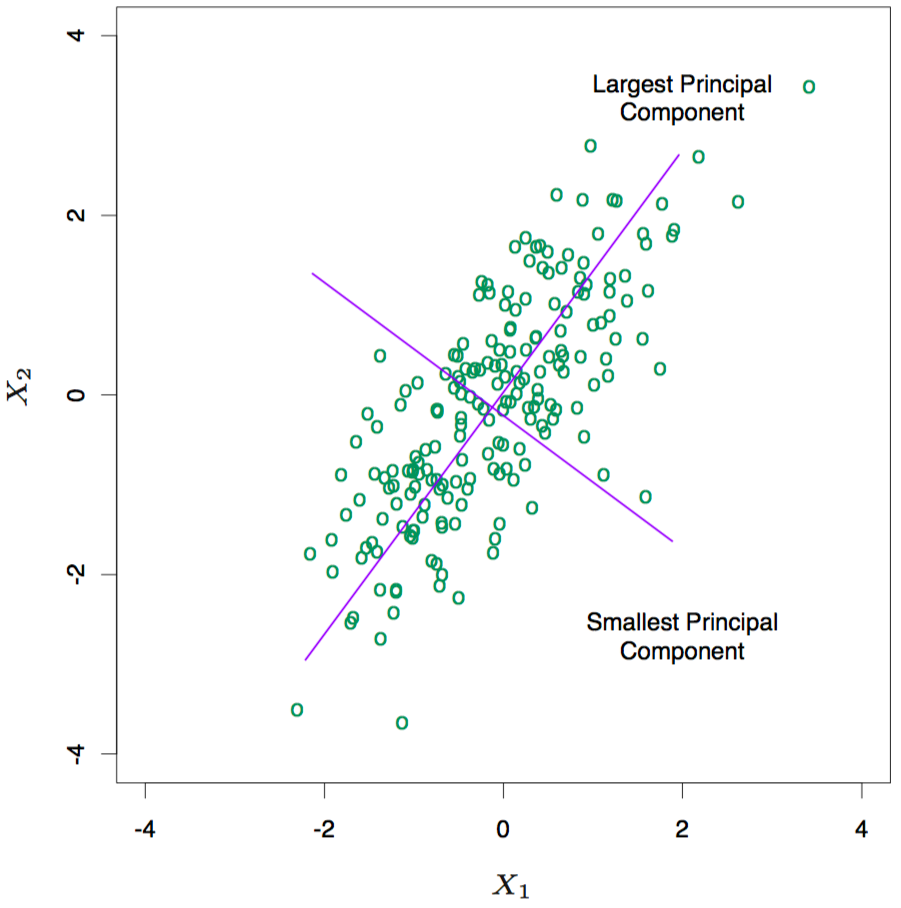
\includegraphics[width=5cm]{pca1.png}
        \end{center}

        % \item For example, the shown below are the high-dimensional MNIST digits projected onto a 2D PCA subspace.
        % \begin{align*}
        % \includegraphics[width=7cm]{pca.png}
        % \end{align*}
        
        \item Let $X \in \mathbb{R}^{n \times d}$ be the data matrix. We first shift the sample mean of each column (i.e. feature) to zero: 
        $$X - \frac{1}{n} \vec{1}_n \vec{1}_n^\top X$$
        because variance is defined relative to the mean of the data. 
        \item Recall the scalar projection of $x \in \mathbb{R}^d$ onto $u \in \mathbb{R}^d$ where $\|u\|=1$ is given by $x^\top u$. We wish to find the direction $u$ that maximizes the variance of the projections of the data points onto $u$. The variance of the projections is given by
        \begin{align*}
        \sum_{i=1}^n (x_i^\top u)^2 = \|Xu\|^2
        \end{align*}
        Hence we desire
        \begin{align*}
        \arg\max_{\| u \| = 1} \| Xu \|^2 &= \arg\max_{\| u \| \neq 0} \frac{\| Xu \|^2}{\| u \|^2} \\
        &= \arg\max_{\| u \| \neq 0} \frac{u^\top X^\top X u}{u^\top u}
        \end{align*}
        This is a Rayleigh quotient, so the maximum possible value is the largest eigenvalue of the matrix $X^\top X$, which occurs when $u$ is the corresponding unit eigenvector. 
        \item To find the $k$-th principal direction, we first subtract off the contributions of the previously computed principal directions $u_1, \hdots, u_{k-1}$:
        \begin{align*}
        \hat{X}_k = X - \sum_{j=1}^{k-1} Xu_j u_j^\top
        \end{align*}
        Then we apply the same rule as before, subject to the constraint that $u_k$ be orthogonal to $u_1, \hdots, u_{k-1}$. These vectors turn out to be the leading $k$ eigenvectors of $X^\top X$. Notice the intimate connection to the SVD of $X$: $U\Sigma V^\top$. The $k$ principal component axes are precisely the first $k$ columns of $V$.
        
        \item Once the principal directions are found, we can use them as a new coordinate system. Each data point $x_i \in \mathbb{R}^d$ becomes a new vector $\hat{x}_i \in \mathbb{R}^k$ such that $[x_i]_j = x_i^\top u_j$. In matrix form, $$\hat{X} = XV$$ where $V \in \mathbb{R}^{d \times k}$ is a matrix whose columns are the principal directions. The data becomes linearly uncorrelated in the PCA coordinate system.
        
        \item Another derivation of PCA comes from a Gaussian assumption. Let us assume the data are generated by a multivariate Gaussian distribution, i.e. $x_i \sim \mathcal{N}(\mu, \Sigma)$. Then the MLE of $\Sigma$ is
        \begin{align*}
        \hat{\Sigma} = \frac{1}{n} \sum_{i=1}^{n} (x_i - \hat{\mu}) (x_i - \hat{\mu})^\top = \frac{1}{n} X^\top X
        \end{align*}
        The contours of the multivariate Gaussian density form ellipsoids, and the direction of largest variance is the eigenvector corresponding to the smallest eigenvalue of $\Sigma^{-1}$, which is the largest eigenvalue of $\Sigma$. Now since the eigenvalues and eigenvectors of $\hat{\Sigma}$ and $X^\top X$ are the same, we arrive at the same solution.
        
        \item It can be shown that minimizing the distance between each $x_i$ and its projection onto $u$ is equivalent to maximizing the projected variance. Thus PCA can be interpreted as minimizing the perpendicular distance between the principal component subspace and the data points. In this sense, it is doing the same thing as total least squares. 
        
        \item Eigenfaces represents a prime example of the usefulness of PCA. After subtracting the ``mean face" from various image samples, we can find the eigenvectors of the covariance matrix, which can be interpreted as eigenfaces. Remarkably, it does not take many eigenfaces combined together to achieve a fair approximation of most faces.
    \end{enumerate}   
    
    \subsection{Canonical Correlation Analysis}
    \begin{enumerate}[label=(\alph*)]
        \item Shown below are various 2D scatterplots with corresponding Pearson correlation coeffcieints:
        \begin{align*}
        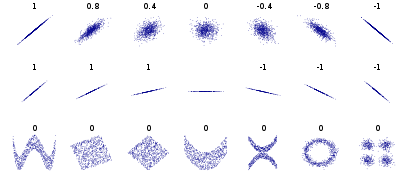
\includegraphics[width=7cm]{corr.png}
        \end{align*}
        \item Given two vectors $X$ and $Y$ of random variables, CCA finds linear combinations of the $X_i$ and $Y_j$ which have maximum correlation with each other. CCA is invariant with respect to scaling or general affine transformations of the variables.
        
        \item Formally, given \textit{zero-mean} random vectors $X_{\text{rv}} \in \mathbb{R}^p$ and $Y_{\text{rv}} \in \mathbb{R}^q$, we seek projection vectors $u \in \mathbb{R}^p$ and $v \in \mathbb{R}^q$ that maximize the correlation $\rho(X_{\text{rv}}^\top u, Y_{\text{rv}}^\top v)$:
        \begin{align*}
            \rho(X_{\text{rv}}^\top u, Y_{\text{rv}}^\top v) 
            &= \frac{\text{Cov}(X_{\text{rv}}^\top u, Y_{\text{rv}}^\top v)}{\sqrt{\text{Var}(X_{\text{rv}}^\top u)\text{Var}(Y_{\text{rv}}^\top v)}} \\
            &= \frac{u^\top \Sigma_{XY} v}{\sqrt{u^\top\Sigma_{XX} u \cdot v^\top \Sigma_{YY} v}}
        \end{align*}
        
        In practice, we estimate the covariance matrices from data. Given paired zero-mean data matrices $X \in \mathbb{R}^{n \times p}$ and $Y \in \mathbb{R}^{n \times q}$, where the rows of $X$ and $Y$ are i.i.d. samples $x_i \in \mathbb{R}^p$ from $X_{\text{rv}}$ and $y_i \in \mathbb{R}^q$ from $Y_{\text{rv}}$, respectively, we have
        \begin{align*}
            \Sigma_{XY} \approx \frac{1}{n} X^\top Y, \hspace{0.2cm}
            \Sigma_{XX} \approx \frac{1}{n} X^\top X, \hspace{0.2cm}
            \Sigma_{YY} \approx \frac{1}{n} Y^\top Y 
        \end{align*}
        
        The problem is then
        $$
        \arg\max_{u,v} \frac{u^\top X^\top Yv}{\sqrt{u^\top X^\top Xu\cdot v^\top Y^\top Yv}}
        $$
        
        \item The first step is to \textit{whiten} $X$ and $Y$ with $W_x$ and $W_y$, with the goal being to make their covariance matrices become the identity. Denote the SVD of $X^\top X = U_x S_x U_x^\top$.
        Choosing $W_x = U_x S_x^{-\frac{1}{2}} U_x^\top$ makes it so that $(X W_x)^\top (X W_x) = I$, as desired. We do the same for $Y$ by choosing $W_y = U_y S_y^{-\frac{1}{2}} U_y^\top$. Since this is an affine transformation, the correlation coefficient remains unchanged. We denote the whitened matrices as $X_w = XW_x$ and $Y_w = YW_y$.
        
        \item Next, we choose matrices $D_x$ and $D_y$ to \textit{decorrelate} $X_w$ and $Y_w$ so that their cross-covariance matrix becomes diagonal. Again, write their SVD:
        $$
        X_w^\top Y_w = U S V^\top
        $$
        Choosing $D_x = U$ and $D_y = V$, we now have
        $$
        (X_w U)^\top  (Y_w V) = U^\top X_w YV = U^\top (U S V^\top) V = S
        $$
        Again, since this is an affine transformation, the correlation coefficient remains unchanged. 
        
        \item Denoting the whitened \textit{and} decorrelated $X$ and $Y$ as $X_d$ and $Y_d$, the optimization problem is now
        \begin{align*}
        \arg\max_{u_d,v_d} \frac{u_d^\top S v_d}{\sqrt{u_d^\top u_d \cdot v_d^\top v_d }}
        \end{align*}
        Without loss of generality, we force $u_d$ and $v_d$ to be unit vectors so that the denominator disappears. The numerator is a sum of the singular values of $S=X_w^\top Y_w$ weighted by $u_d$ and $v_d$, which is maximized by extracting the maximal singular value, i.e. 
        $$
        u_d = v_d = \begin{bmatrix} 1 & 0 & \cdots & 0 \end{bmatrix}
        $$
        Finally, we have
        $$
        u = W_x D_x u_d, \hspace{10pt} v = W_y D_y v_d
        $$
        
        \item More generally, to obtain the $k$ best directions, we choose $U_d \in \mathbb{R}^{p \times k}$ to be the $k$-dimensional identity matrix with $p-k$ rows of zero added to the bottom, and $V_d \in \mathbb{R}^{q \times k}$ to be the $k$-dimensional identity matrix with $q-k$ rows of zero added to the bottom.
        Then
        \begin{align*}
            U = W_x D_x U_d, \hspace{1cm} V = W_y D_y V_d
        \end{align*}
        for $U \in \mathbb{R}^{p \times k}$ and $V \in \mathbb{R}^{q \times k}$.
        
        \item An application of CCA is regression. Let the projected data matrcies be $X_c = XU$ and $Y_c = YV$. We can fit a linear model relating the two: $Y_c \approx X_c A$, where $A\in \mathbb{R}^{k \times k}$, which can be solved by OLS. Through a series of transformations, we can eventually form a matrix that gives the prediction $\hat{Y}$ from (new) zero mean observations $X$.
        
        \item In summary, CCA simultaneously finds projection directions in the two spaces such that the projected data have maximal correlation, whereas PCA defines a new orthogonal coordinate system that optimally describes variance in a single dataset. Both are common methods of dimensionality reduction.
    \end{enumerate}       

\end{addmargin}

\section{Nonlinear Regression and Neural Nets}
\begin{addmargin}[0.8em]{0.5em}

    \subsection{Nonlinear Least Squares}
    \begin{enumerate}[label=(\alph*)]
        \item All the models we’ve seen so far are linear in the parameters we’re trying to learn. We consider the optimization problem
        $$
        \arg\min_{\theta} \sum_{i=1}^n (y_i - f(x_i; \theta))^2
        $$
        except now, $f$ is nonlinear. There is no closed-form solution, but there are iterative methods.
        \item One such method is the Gauss-Newton algorithm. At each iteration, this method linearly approximates the objective function with a first-order Taylor expansion about the current iterate: $F(\theta) \approx F(\theta^{(k)}) + J(\theta^{(k)}) \Delta \theta$.
        Since this is linear in $\Delta \theta$, so we solve a least-squares problem involving the linearized objective in order to compute the next iterate. 
        The process is as follows:
        \begin{enumerate}[1.]
        \item Initialize $\theta^{(0)}$ with some guess
        \item Repeat until convergence:
        \begin{enumerate}
        \item Compute Jacobian with respect to the current iterate: $J = J(\theta^{(k)})$
        \item Compute $\Delta Y = Y - F(\theta^{(k)})$ 
        \item Update $\theta^{(k+1)} = \theta^{(k)} + (J^\top J)^{-1} J^\top \Delta Y$
        \end{enumerate}
        \end{enumerate}
    \end{enumerate}  

    \subsection{Gradient Descent}

    \begin{enumerate}[label=(\alph*)]
        \item Gradient descent is an iterative optimization algorithm for finding the minimum of a function. We take steps proportional to the negative of the gradient of the function at the current point. That is, starting from an intial point $x_0$, we repeat
        $$x_{i+1} = x_i - \gamma_i \nabla f(x_i)$$
        for some step size $\gamma$, which may be constant or decrease over iterations.
        \vspace{-0.2cm}
        \begin{center}
            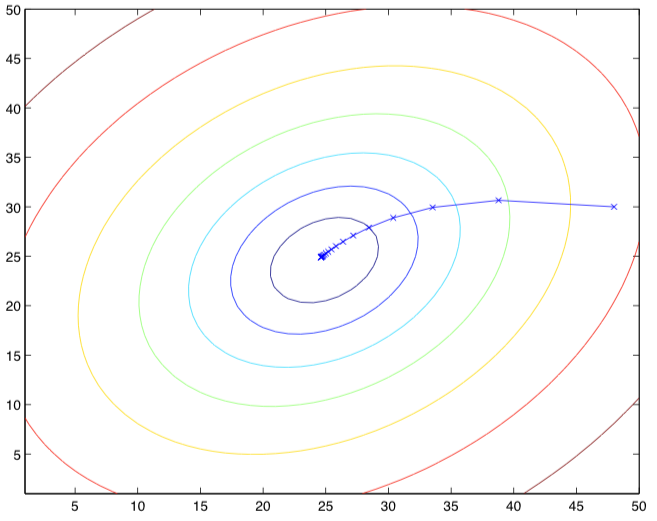
\includegraphics[width=4.4cm]{gd.png}
        \end{center}
        \vspace{-0.4cm}
        
        \item The function $\| Ax - b \|_2$ is convex, but convergence requires care and is exponential in $\|b\|_2$. For the quadratic function $\frac{1}{2} \| Ax - b\|_2^2$, we show that we have \textit{geometric} convergence. In the case $\|b\|=\vec{0}$, we write
        \begin{align*}
        x_{i+1} = x_i - \gamma (A^\top A x_i - A^\top b) = (I - \gamma A^\top A)x_i
        \end{align*}
        by induction,
        \begin{align*}
        x_{i+1} = (I - \gamma A^\top A)^{i+1}x_0
        \end{align*}
        Note that 
        \begin{align*}
        \| (I - \gamma A^\top A)^{k}v \|_2 \leq (| \lambda_{\text{max}}(I - \gamma A^\top A) |)^k \|v\|_2
        \end{align*}
        so that this state evolution is stable only if the eigenvalues of $(I - \gamma A^\top A)$ are bounded by (in absolute value) 1.
        
        For general $b$, after $k$ steps of gradient descent with some constant step size $\gamma > 0$,
        \begin{align*}
        f(x_k) - f(x^*) \leq \frac{\alpha}{2} \beta^{2k} \|x_0-x^*\|_2^2
        \end{align*}
        where $\alpha = \lambda_{\max}(A^TA)$ and $\beta = \max \{ | 1 - \gamma \lambda_{\max}(A^TA) |, | 1 - \gamma \lambda_{\min}(A^TA) | \}$. If we choose $\gamma$ to make $\beta$ as small as possible:
        $$\gamma = \frac{2}{\lambda_{\max}(A^TA) + \lambda_{\min}(A^TA)} $$
        then the convergence rate can be written
        \begin{align*}
        f(x_k) - f(x^*) \leq \frac{\alpha}{2} \left( \frac{Q-1}{Q+1} \right)^{2k} \|x_0-x^*\|_2^2
        \end{align*}
        where $Q = \lambda_{\max}(A^TA) / \lambda_{\min}(A^\top A)$, the condition number of $A^\top A$.
    \end{enumerate}
    
    \subsection{Neural Networks}
    \begin{enumerate}[label=(\alph*)]
        \item An \textit{artificial neural network} is a collection of connected units (neurons) that can transmit a signal from one to another. The signal is a real number, and the output of each neuron is calculated by a non-linear function of the sum of its input. 
        
        \item Each neuron receives an input vector $x$ and computes $z = w^\top x + b$ , where $w$ is a vector of weights and $b$ is a bias term. The output is computed $a=g(z)$, where $g$ is some activation function. Example activation functions include:
        \begin{itemize}
        \item $g(z) = \frac{1}{1 + e^{-z}}$ (sigmoid)
        \item $g(z) = \max(z,0)$ (ReLU)
        \item $g(z) = \frac{e^z - e^{-z}}{e^z + e^{-z}}$ (tanh)
        \end{itemize}
        
        \item Non-linearity gives neural networks their representational power, as the output we are trying to predict often has a non-linear relationship with the inputs. Without non-linear activation functions, the neural network simply performs linear regression.        
        
        \item ReLU activations are very common for intermediate layers of neural nets in practice. The \textit{universal approximation theorem} states that for every continuous function $f$ on a closed and bounded subset $S$, there exists a neural network with one (finite) hidden layer that uniformly approximates $f$ on $S$, under mild assumptions on the activation function.
        \columnbreak
        
        \item Consider the following simple network:
        \begin{center}
            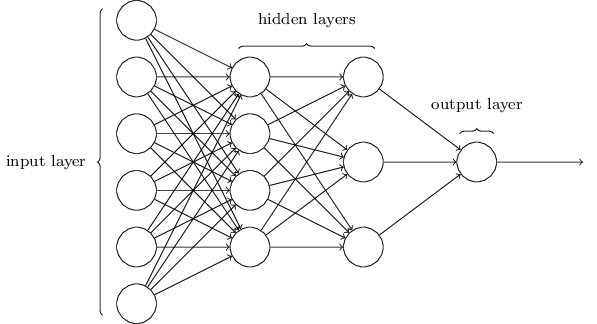
\includegraphics[width=7.5cm]{nn.png}
        \end{center}
        Denote the input layer as layer 0, the first hidden layer as layer 1, and so on. Let $a_j^{[\ell]}$ denote the activation of the $j$th unit of layer $\ell$. The first unit in layer 1, for instance, performs 
        $$z_1^{[1]} = {W_1^{[1]}}^\top x + b_1^{[1]} \text{ and } a_1^{[1]} = g(z_1^{[1]})$$ 
        where ${W_1^{[1]}}^\top$ is the first row of $W^{[1]}$, the weight matrix of layer 1.
        
        The output computation of layer 1 can be vectorized as follows:
        \begin{align*}
            \underbrace{ 
            \begin{bmatrix}
            z_1^{[1]} \\ \vdots \\ z_4^{[1]}
            \end{bmatrix} 
            }_{
            z^{[1]} \in \mathbb{R}^{4}
            }
            =
            \underbrace{ 
            \begin{bmatrix}
            \text{--- }  {W_1^{[1]}}^\top  \text{---} \\
            \vdots  \\
            \text{--- }  {W_4^{[1]}}^\top  \text{---} \\
            \end{bmatrix} 
            }_{
            W^{[1]} \in \mathbb{R}^{4 \times 6}
            }    
            \underbrace{ 
            \begin{bmatrix}
            x_1 \\ \vdots \\ x_6
            \end{bmatrix} 
            }_{
            x \in \mathbb{R}^{6}
            }           
            +
            \underbrace{ 
            \begin{bmatrix}
            b_1^{[1]} \\ \vdots \\ b_4^{[1]}
            \end{bmatrix} 
            }_{
            b^{[1]} \in \mathbb{R}^{4}
            }            
        \end{align*}
        Next, $a^{[1]} = g(z^{[1]})$, which can be performed quickly by parallel element-wise operations. The output of layer 1, $a^{[1]}$, becomes the input to layer 2.
        
        These operations can also be vectorized over training samples. Given $n$ training samples $x^{(i)} \in \mathbb{R}^6$, define
        $
            X = 
            \begin{bmatrix} 
            | & & | \\
            x^{(1)} & \cdots & x^{(n)} \\
            | & & |
            \end{bmatrix}
        $.
        Then we have
        \begin{align*}
            Z^{[1]} =
            \begin{bmatrix} 
            | & & | \\
            z^{[1](1)} & \cdots & z^{[1](n)} \\
            | & & |
            \end{bmatrix}
            = W^{[1]} X + b^{[1]}
        \end{align*}      
        Similarly, $A^{[1]} = g(Z^{[1]})$ is obtained by element-wise operation $g$ on the matrix $Z^{[1]}$. This forward propagation process continues until the output layer. 
        
        \item The nonlinearities $g$ are typically the same for all layers except the last. This is because the output layer may be doing regression (e.g. linear), binary classification (e.g. sigmoid) or multiclass classification (e.g. softmax).
        
        \item Neural networks with multiple hidden layers are called deep neural networks. Such networks discover complex features useful for predicting the output, but are often difficult to interpret. Choosing an appropriate architecture is very much trial-and-error.     
    \end{enumerate}
    \vspace{-0.3cm}
    \subsection{Backpropagation}
    \begin{enumerate}[label=(\alph*)]
        \item Parameters (weights and biases) are learned by performing gradient descent on a loss function. \textit{Backpropagation} is a method of calculating these gradients by using the chain rule to iteratively compute gradients at each layer.
        
        \item It is important to randomly initialize the parameters to small values (so that the gradients will be different and the nuerons learn different features).        
        
        \item The first step is the forward pass, as discussed earlier. For a network with $M$ layers, we define $x=a^{[0]}$ and compute up to $\hat{y}=a^{[M]}$, saving the intermediate results in the process. We measure the error with a loss function $\mathcal{L}(\hat{y}, y)$, where $y$ is the desired output. For example, in regression we might use
        $\mathcal{L}(\hat{y}, y) = \frac{1}{2} \| \hat{y} - y \|_2^2$.
        
        \item Now define 
        $$
        \delta^{[\ell]} = \frac{\partial \mathcal{L}}{\partial z^{[\ell]}}
        $$
        \begin{enumerate}[1.]
            \item For output layer $M$, we have
            $$
            \delta^{[M]} = \frac{\partial \mathcal{L}}{\partial z^{[M]}}
            $$
            \item For $\ell=M-1, \hdots, 1$ we have
            $$
            \delta^{[\ell]} = ({W^{[\ell + 1]}}^\top \delta^{[\ell + 1]}) \circ g'(z^{[\ell]})
            $$
            where $\circ$ denotes the elementwise product.
            \item Finally, compute the gradients for layer $\ell$ as
            \begin{align*}
                \frac{\partial \mathcal{L}}{\partial W^{[\ell]}} &= \delta^{[\ell]} {a^{[\ell - 1]}}^\top \\
                \frac{\partial \mathcal{L}}{\partial b^{[\ell]}} &= \delta^{[\ell]} 
            \end{align*}
        \end{enumerate}
        We repeat the above procedure for all $n$ training samples, then apply the averaged gradient descent update to each layer $\ell$:
        \begin{align*}
            W^{[\ell]} &= W^{[\ell]} - \frac{\gamma}{n} \sum_{i=1}^{n} \frac{\partial \mathcal{L}^{(i)}}{\partial W^{[\ell]}} \\
            b^{[\ell]} &= b^{[\ell]} - \frac{\gamma}{n} \sum_{i=1}^{n} \frac{\partial \mathcal{L}^{(i)}}{\partial b^{[\ell]}} 
        \end{align*}
        where $\gamma$ is the learning rate and $\mathcal{L}^{(i)}$ is the loss for a single instance. Note that the above procedure can also be vectorized over training samples.
        
        \item Computing gradients over all $n$ data points is costly. In practice, the loss gradient is approximated over a \textit{mini-batch} of $m$ data points. This method is called \textit{stochastic gradient descent} (SGD). In a single \textit{epoch}, backpropogation is run $n/m$ times, with each run updating parameters over the batch average.
        
        \item Training deep networks is an area of active research. Topics of interest include parameter initialization, regularization (e.g. dropout), choosing an appropriate learning schedule, and speeding up convergence (e.g. SGD with momentum). 
    \end{enumerate} 
    \vspace{-0.6cm}
\end{addmargin}

\section{Classification}

\begin{addmargin}[0.8em]{0.5em}
    \subsection{LDA and QDA}
    \begin{enumerate}[label=(\alph*)]
        \item The task of classification differs from regression in that the goal is to assign a data point to a discrete number of classes instead of a continuous value.
        
        \item Given a training set $\{ (x_i, y_i) \}_{i=1}^{n}$ of paired data points $x_i \in \mathbb{R}^d$ and discrete class label $y_i \in \{ 1, \hdots, K \}$, the goal of a classifier is to assign an arbitrary data point $X$ to one of the $K$ discrete classes.
        
        \item There are two main types of models that can be used to train classifiers: generative and discriminative models. Generative models involve explicitly forming:
        \begin{enumerate}[1.]
            \item A prior probability distribution over all classes $k \in \{ 1, \hdots, K \}$:
            $$
            P(k) = P(\text{class} = k)
            $$
            \item A conditional probability distribution for each class $k$:
            $$
            f_k(X) = f(X | \text{class}= k)
            $$
        \end{enumerate}
        Using Bayes' rule, the predicted class label $k^*$ is then
        \begin{align*}
            k^* = \arg\max_{k} P(\text{class}=k | X) = \arg\max_{k} f_k(X) P(k)
        \end{align*}
        
        \item \textit{Quadratic discriminant analysis} (QDA) is a generative method in which the class conditional probability distributions are assumed to be independent Gaussians: $f_k \sim \mathcal{N}(\mu_k, \Sigma_k)$. The means and covariances $\mu_k, \Sigma_k$ are typically empirically estimated using MLE (see appendix).
        
        \item The predicted class label $k^*$ is given by $k^* = \arg\max_{k} f_k(X) P(k)$. We have $\log{f_k(X) P(k)}$
        \begin{align*}
        = -\frac{1}{2} (X - \mu_k)^\top \Sigma_k^{-1} (X - \mu_k) - \frac{1}{2} \log{|\Sigma_k|} + \log{P(k)}
        \end{align*}
        The decision boundary separating two classes is a quadratic function of $X$, hence the name.
        
        \item If we assume that all classes have the same covariance matrix $\Sigma$, we have \textit{linear discriminant analysis} (LDA). This time, $\Sigma$ is empirically estimated using \textit{all} training samples.
        
        \item We have
        \begin{align*}
        \log{f_k(X) P(k)} &= -\frac{1}{2} (X - \mu_k)^\top \Sigma^{-1} (X - \mu_k) + \log{P(k)} \\
        &= X^\top \Sigma^{-1} \mu_k - \frac{1}{2} \mu_k^\top \Sigma^{-1} \mu_k + \log{P(k)}
        \end{align*}
        The decision boundary between class $k$ and $l$ is then
        \begin{align*}
        X^\top \Sigma^{-1} (\mu_k - \mu_l) - \frac{1}{2} (\mu_k + \mu_l)^\top \Sigma^{-1} (\mu_k - \mu_l) + \log{\frac{P(k)}{P(l)}}
        \end{align*}
        equated to zero. The decision boundary is now a linear function of $X$. In the binary case (say $k=1$, $l=2$), we classify $X$ as $1$ if $X^\top w > c$ and 2 otherwise, where
        \begin{align*}
        w &= \Sigma^{-1}(\mu_1 - \mu_2) \\
        c &= \frac{1}{2} (\mu_1 + \mu_2)^\top \Sigma^{-1} (\mu_1 - \mu_2) + \log{\frac{P(1)}{P(2)}}
        \end{align*}
        
        \item We could also perform MLE by not using prior terms. Notice that uniform priors reduce to MLE. 
        
        \item An example of LDA (left) and QDA (right) boundaries is shown below.
        \begin{center}
            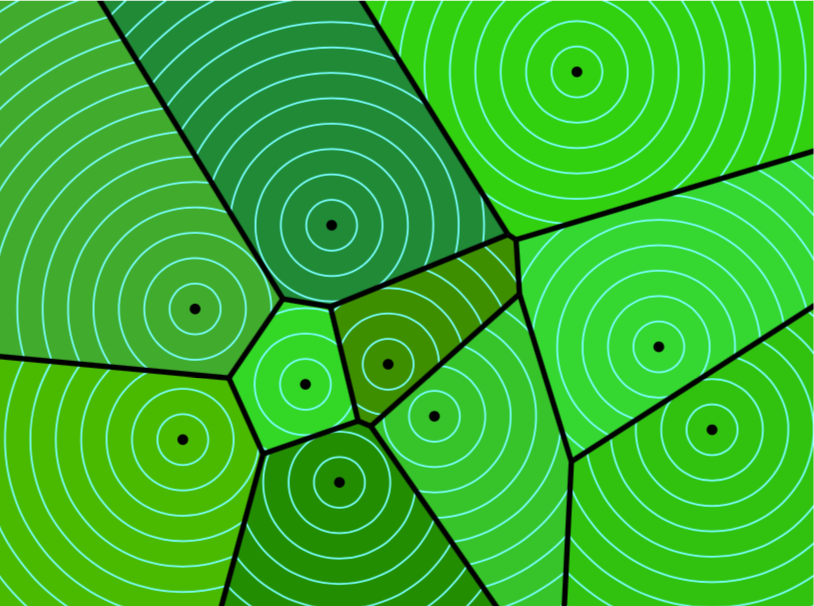
\includegraphics[width=3.8cm]{lda1.png}
            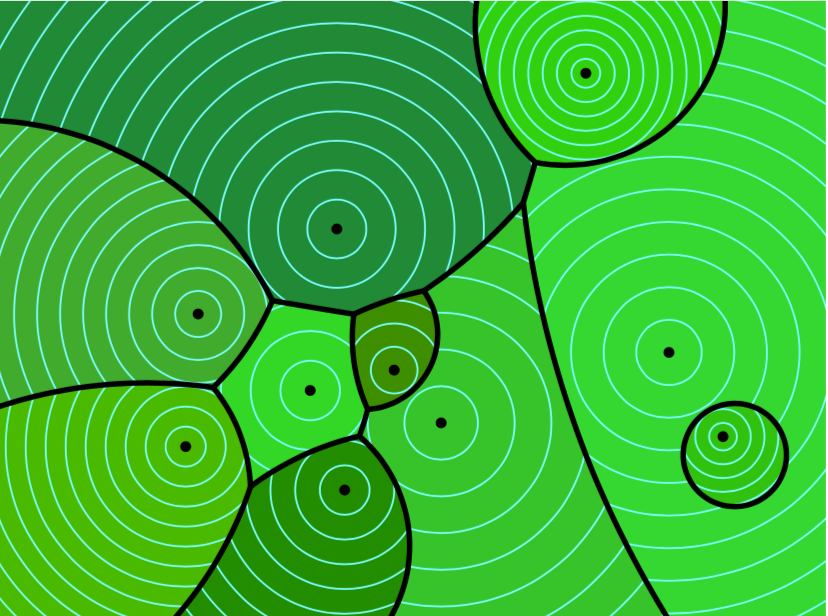
\includegraphics[width=3.8cm]{qda1.png}
        \end{center}
    \end{enumerate}
    
    \subsection{Logistic Regression}
    \begin{enumerate}[label=(\alph*)]
        \item Generative models (e.g. QDA, LDA) can be inefficient in that they require estimation of a large number of parameters. Discriminative models, in contrast, attempt to model the posterior directly.
       
        \item We start with the case of binary classification, i.e. $y_i \in \{-1, 1\}$. We could apply standard linear regression to learn parameters $w \in \mathbb{R}^{d+1}$ and classify $x$ to be $\text{sign}(w^\top x)$. (Note that we add an extra feature of 1 to $x$ so as to absorb the bias term into $w$) We could optimize $w$ as follows:
        $$
        \arg\min_w \sum_{i=1}^n \| y_i - w^\top x_i \|_2^2 + \lambda \| w \|_2^2
        $$
        This method is called the 2-class least squares support vector machine (LS-SVM). However, it is easy to construct examples where this method performs very poorly. 
        \item \textit{Logistic regression} is a discriminative classification technique with a probabilistic interpretation. This time, we assume $y_i \in \{0, 1\}$. We first convert the linear function $w^\top x$ into a probability by applying the sigmoid function $\sigma(z) = \frac{1}{1+e^{-z}}$ (shown below).
        \begin{center}
            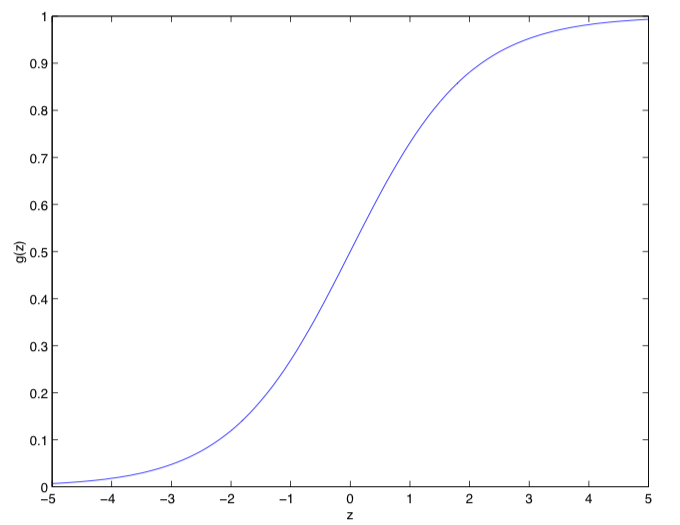
\includegraphics[width=3.5cm]{sigmoid.png}
        \end{center}
        The decision rule for $x_i$ is then
        \begin{align*}
            \hat{y_i} = 
            \begin{cases}
            1 \text{ if $w^\top x_i \geq 0$} \\
            0 \text{ otherwise}
            \end{cases}
        \end{align*}
        We optimize $w$ by minimizing the cross-entropy, or logistic, loss function:
        $$
        \mathcal{L}(w) = \sum_{i=1}^n  y_i \ln \left( \frac{1}{p_i} \right) + (1 - y_i) \ln \left( \frac{1}{1 - p_i} \right)
        $$
        where $p_i = \sigma(w^\top x_i)$.
        \item One way of deriving the cross-entropy loss is via MLE. For the dataset $\{ (x_i, y_i) \}_{i=1}^{n}$, where each sample $Y_i \sim \textit{Bernoulli}(p_i)$, we can write the likelihood of a single data point as $$P(Y_i = y_i) = p_i^{y_i} (1 - p_i)^{(1-y_i)}$$
        Then $\arg\max_w \prod_{i=1}^{n} P(Y_i = y_i)$ is equivalent to the cross-entropy formulation above.
        
        \item The cross-entropy loss can also be derived from an information-theoretic perspective. It minimizes the Kullback-Leibler (KL) divergence, which measures how much a distribution diverges from another.
        
        \item Now we turn to multiclass logistic regression. A common representation is \textit{one-hot vector encoding}. If the $i$th training sample has class $k$, we use the representation $y_i = e_k$, the $k$th canonical basis vector. Now we have a weight matrix $W \in \mathbb{R}^{K \times d+1}$; to classify a data point $x_i \in \mathbb{R}^{d+1}$, we compute $Wx_i$ and choose the index of the largest component.
        
        Each data point $x_i \in \mathbb{R}^{d+1}$ is given a score $z_k = w_k^\top x_i$, where $w_k^\top$ is the $k$th row of $W$. The generalization of the logistic function for the multiclass setting is the softmax function:
        $$
        \text{softmax}(j, z_1, \hdots, z_K) = \frac{e^{z_j}}{\sum_{k=1}^K e^{z_k}}
        $$
        It outputs the probability that the corresponding softmax distribution takes value $j$.
        The multiclass loss function is
        \begin{align*}
            \mathcal{L}(W) = -\sum_{i=1}^{n}\sum_{j=1}^{K} 1\{ y_i = j \} \ln \left( \frac{e^{w_j^\top x_i}}{\sum_{k=1}^K e^{w_k^\top x_i }} \right)
        \end{align*}
        which, again, comes from MLE or KL divergences.
        
        \item The logistic regression loss function has no closed-form solution, so it is typically minimized with SGD. For binary classification, we have
        $$
        \nabla_w \mathcal{L}(w) = -\sum_{i=1}^{n} (y_i - p_i)x_i
        $$
    \end{enumerate}    
    % \vspace{-0.8cm}
    \subsection{Support Vector Machines}
    \vspace{-0.2cm}
    \begin{enumerate}[label=(\alph*)]
        \item \textit{Support Vector Machines} (SVMs) are an attempt to model decision boundaries directly without modeling any probabilities. Formally, we have the data set $\{ (x_i, y_i) \}_{i=1}^{n}$, where $x_i \in \mathbb{R}^d$ and $y_i \in \{-1,1\}$. The goal is to find a $d-1$ dimensional hyperplane decision boundary separating the two classes. They are extensions of the simpler perceptron classifier. They fix many of its shortcomings, namely finding a best-fit boundary even if the data is not linearly separable, and finding the ``best" possible boundary. 
        
        \item Hard-Margin SVMs maximize the margin, or the minimum distance from the decision boundary to any of the training points. Intuitively, maximizing the margin allows the classifier to generalize better to unseen data. The linear decision boundary is the hyperplane $H = \{x \mid w^\top x = t \}$, where $w$ is normal to $H$. Note that the distance between hyperplanes $H_1: w^\top x = a$ and $H_2: w^\top x = b$ is $\frac{|a-b|}{\|w\|_2}$.
        \begin{center}
            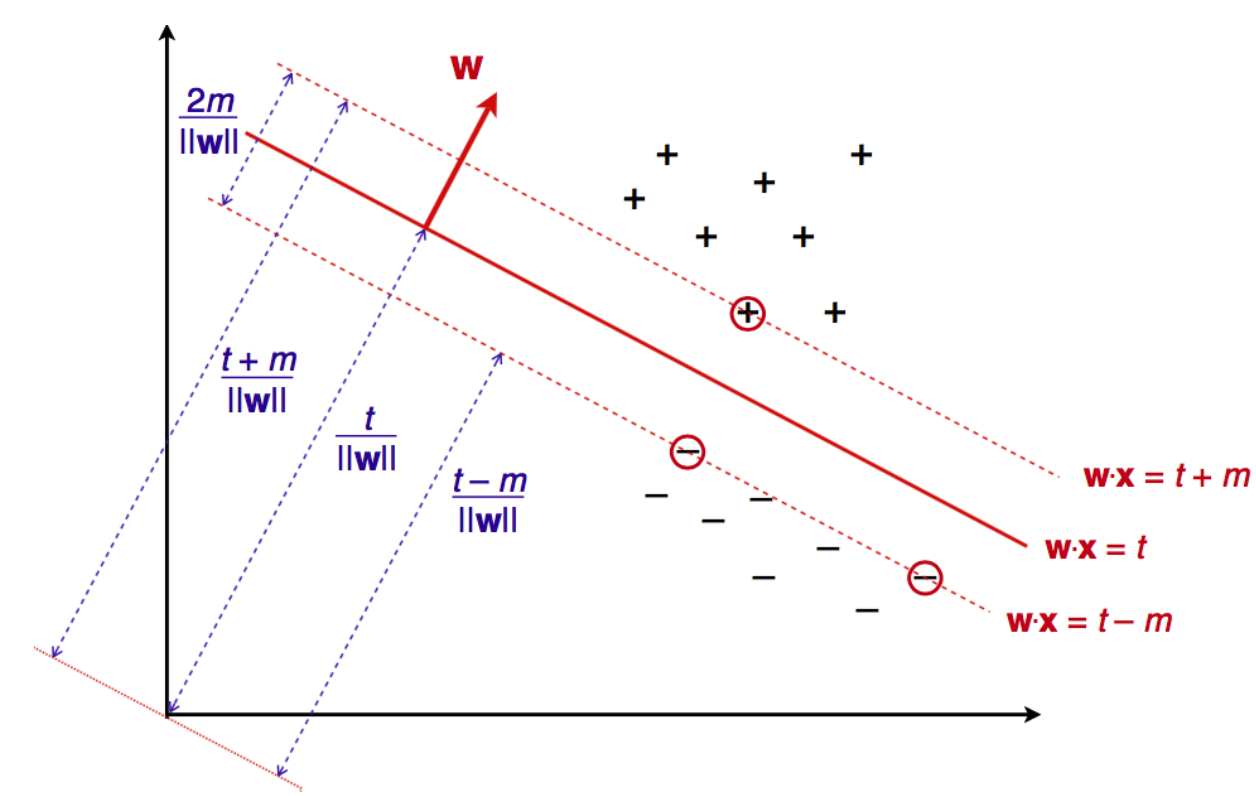
\includegraphics[width=6cm]{svm.png}
        \end{center}
        We wish to maximize the margin $\frac{2m}{\| w \|_2}$. We can freely rescale $t, \|w\|_2, m$, so we set $m=1$. Maximizing the margin then corresponds to minimizing $\|w\|_2$, or more conveniently, $\frac{1}{2} \|w\|_2^2$. 
        \begin{align*}
            \min_{w, t} \frac{1}{2} \|w\|_2^2 \\
            \text{s.t. } y_i(w^\top x_i - t) \geq 1 \, \forall i
        \end{align*}
        The hyperplane is completely determined by those $x_i$ which lie nearest to it. These points are called \textit{support vectors}.
        
        \item The hard-margin SVM optimization problem has a solution only if the data are linearly separable. In addition, it is senstive to outliers. A \textit{soft-margin} SVM modifies the constraints from the hard-margin SVM by allowing some points to violate the margin. It introduces \textit{slack variables} $\xi_i$ for each training point so that each $x_i$ need only be a distance of $1-\xi_i$ from the hyperplane. The soft-margin SVM optimization problem is
        \begin{align*}
            \min_{w, t, \xi_i} \frac{1}{2} \|w\|_2^2 &+ C\sum_{i=1}^{n} \xi_i \\
            \text{s.t. } y_i(w^\top x_i - t) &\geq 1 - \xi_i \, \forall i \\
            \xi_i &\geq 0 \, \forall i
        \end{align*}
        
        Here $C$ is a hyperparameter. A large $C$ keeps $\xi_i$'s small, but may lead to overfitting; a small $C$ is less sensitive to outliers, but may lead to underfitting.
        
        \item The soft-margin SVM is an example of an \textit{empirical risk minimization} (ERM) algorithm. Regularized ERM algorithms are a family of learning methods of the form
        \begin{align*}
            \min_f \frac{1}{n} \sum_{i=1}^{n} \mathcal{L}(y_i, f(x_i)) + \lambda \| f \|^2
        \end{align*}
        (called Tikhonov regularization). It can be shown that the soft-margin SVM optimization problem is equivalent to
        \begin{align*}
            \min_{w,t} \frac{1}{n} \sum_{i=1}^{n} \max(1 - y_i(w^\top x_i - t), 0) + \lambda \|w\|_2^2
        \end{align*}
        for $\lambda=\frac{1}{2Cn}$. Hence soft-margin SVM is regularized empirical risk minimization with the \textit{hinge loss}.
        \begin{center}
            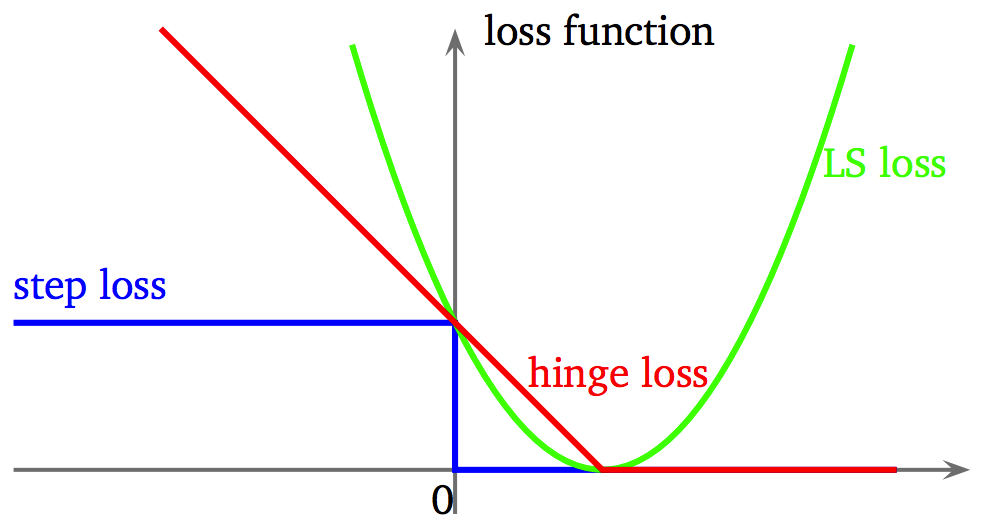
\includegraphics[width=4.2cm]{erm.png}
        \end{center}
        From this perspective, SVM is closely related to other fundamental classification algorithms such as regularized least squares and logistic regression. The difference lies in the choice of loss function: square-loss for LS and log-loss for logistic.
        
        \item The classical approach to solving SVMs involves reducing the optimization problem to its dual, a quadratic programming problem. While the primal SVM finds two parallel bounding planes of maximum separation, the dual SVM finds the closest points between two convex hulls. It can be shown that the Lagrangian dual is given by
        \begin{align*}
            \max_{\alpha} \alpha^\top \vec{1} - \frac{1}{2} \alpha^\top G \alpha \\
            \text{ where } G_{ij} = y_i(x_i^\top x_j) y_j \\
            \text{s.t. } \sum_{i=1}^{n} \alpha_i y_i = 0 \, \forall i \\
            0 \leq \alpha_i \leq C \, \forall i
        \end{align*}
        The dual variables $\alpha_i$ have the following meaning: 
        \begin{center}
            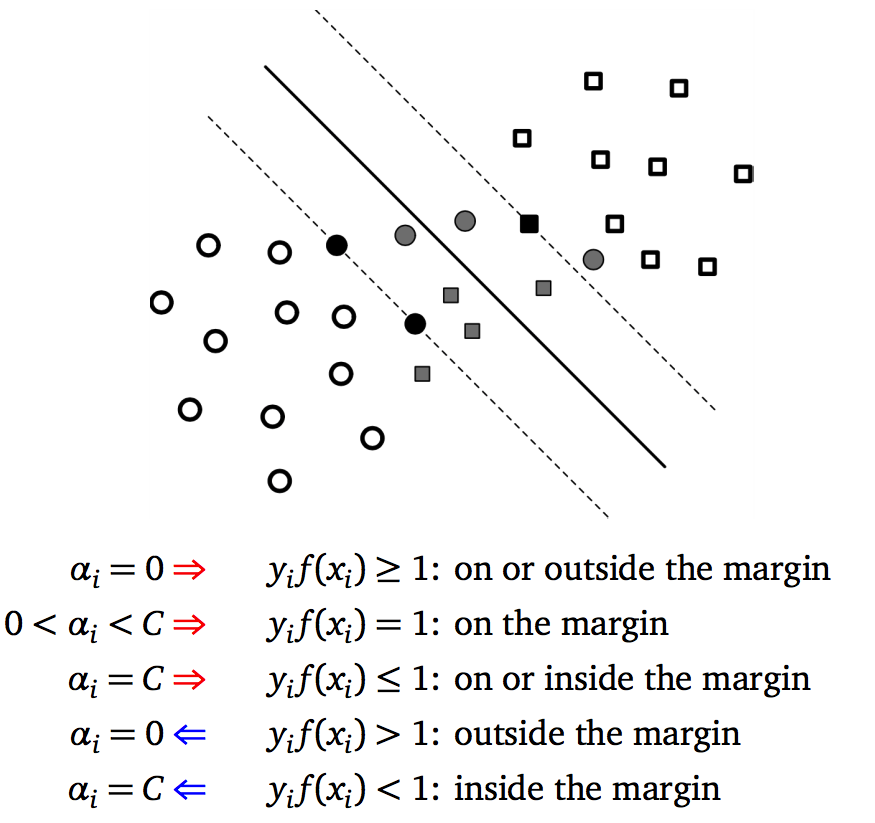
\includegraphics[width=5cm]{dualsvm.png}
        \end{center}
        The primal values can be reconstructed as follows:
        \begin{align*}
            w &= \sum_{i=1}^{n} \alpha_i y_i x_i \\
            t &= \text{mean}(w^\top x_i \hspace{0.4cm} \forall i: 0 < \alpha_i < C) \\
            \xi_i &= 
            \begin{cases}
            1 - y_i(w^\top x_i - t) \text{ if } \alpha_i = C \\
            0 \text{ otherwise }
            \end{cases}
        \end{align*}
        
        \item Multiclass SVM is typically done with multiple binary SVM classifiers between one of the labels and the rest (one vs all), or between every pair of classes (one vs one).
    \end{enumerate}    
    
    \subsection{Kernel Methods}
    \begin{enumerate}[label=(\alph*)]
        \item Recall in regression we often augment the original input $x$ using a feature mapping $\phi(x)$. We can run SVM on the transformed data points to learn a nonlinear decision boundary, which corresponds to a linear boundary in the augmented feature space.
        
        \item The dual SVM solution can be written entirely in terms of inner products $\langle x_i, x_j \rangle = x_i^\top x_j$. We can replace each inner product with a \textit{kernel function}:
        $$
        k(x_i, x_j) = \langle \phi(x_i), \phi(x_j) \rangle
        $$
        A valid kernel is a function $k$ that can be expressed as an inner product of feature maps $\phi$. Equivalently, $k$ is a valid kernel if the corresponding kernel matrix $K$, where $K_{ij} = k(x_i, x_j)$, is positive semi-definite.
        
        \item The power of kernels comes from the fact that we can define a kernel $k$ without an explicit representation for $\phi$. By Mercer's theorem, an implicitly defined function $\phi$ exists for any suitable $k$. This is useful because $k(x_i, x_j)$ may be inexpensive to calculate, whereas the corresponding $\phi(x_i), \phi(x_j)$ may be very expensive to calculate.
        
        \item For example, the polynomial kernel $k(x_i, x_j) = (x_i^\top x_j + c)^d$ corresponds to a feature mapping to a $\binom{n+d}{d}$-dimensional feature space. Still, computing $k(x_i, x_j)$ takes only $O(n)$ time even though the feature vectors lie in $O(n^d)$ dimensional space (where $n$ is the dimension of the original data).
        
        \item Another popular kernel is the Gaussian radial basis function:
        $$
        k(x_i, x_j) = \exp \left( -\frac{\| x_i - x_j \|^2}{2\sigma^2} \right)
        $$
        which corresponds to an \textit{infinite}-dimensional feature mapping $\phi$. A larger $\sigma$ results in a smoother boundary (less variance).
        
        \item After training kernel SVM, a new point $x$ can be classified by computing the sign of
        \begin{align*}
            w^\top \phi(x) - t &= \left( \sum_{i=1}^{n} \alpha_i y_i x_i \right)^\top \phi(x) - t \\
            &= \sum_{i=1}^{n} \alpha_i y_i (x_i^\top x) - t
        \end{align*}
        We do this so as to avoid forming $\phi(x)$. So while linear SVM needs only store the vector $w$ for testing, kernel SVM needs to store all support vectors ($x_i$ for which $\alpha_i > 0$) for testing.
        
        \item The ``kernel trick" can be applied to many machine learning algorithms that only involve inner products of training samples, including linear and ridge regression, logistic regression, and PCA.
        
        \item For example, consider kernel ridge regression. Let $X \in \mathbb{R}^{n \times d}$ be the feature matrix such that the $i$th row is $\phi(x_i) \in \mathbb{R}^d$. We decompose $w \in \mathbb{R}^d$ into $X^\top w_1 + w_2$, where $w_1 \in \mathbb{R}^n$ and $w_2 \in \mathcal{N}(X)$. The solution is given by
        $$
        w = X^\top (XX^\top + \lambda I)^{-1} y
        $$
        which can be shown to be equivalent to the original ridge regression solution. Predicting a new output $\hat{y}$ from $x$ is computed with
        \begin{align*}
            \hat{y} = \langle \phi(x), w \rangle = \begin{bmatrix} k(x_1, x)  \hdots  k(x_n, x) \end{bmatrix}^\top (K + \lambda I)^{-1} y
        \end{align*}
        where $K$ is the corresponding kernel matrix (observe we never actually need to go to the feature space). 
        
        \item Kernelized methods are computationally preferable if $d \gg n$, i.e., the number of features far exceeds the number of training samples.
    \end{enumerate}     
    
    \subsection{Nearest Neighbor Classifiers}
    \begin{enumerate}[label=(\alph*)]
        \item The $k$-nearest neighbors (kNN) classifier assumes data points that are sufficiently close to one another should be of the same class. To predict on a test data point $x$, we compute the $k$ nearest training data points to $x$, where ``closeness" is quantified in some distance function (e.g. Euclidean distance). Then we classify $x$ by a majority vote of its neighbors. 
        \item $k$-nearest neighbors can also be used to perform regression; we instead return the (weighted) average of the values of its $k$ nearest neighbors.
        
        \item kNN can produce complex nonlinear decision boundaries for large $k$. For example, the decision boundary for a 15-NN classifier with 2 classes is shown below.
        \begin{center}
            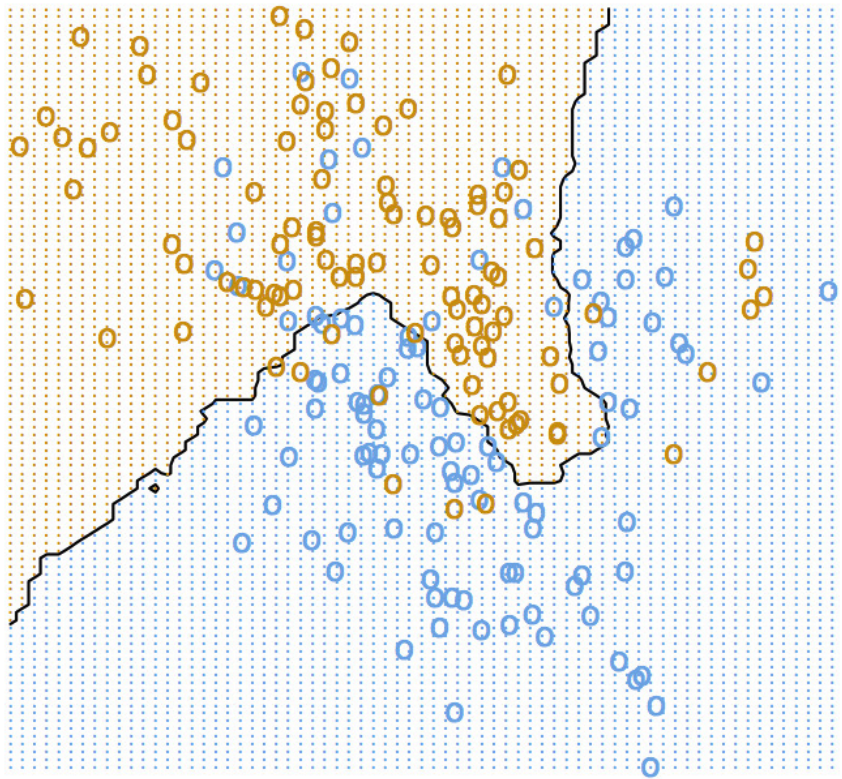
\includegraphics[width=5cm]{knn2.png}
        \end{center}
        
        \item A kNN classifier does not need to be trained. However, for $n$ training samples, the classifer requires $O(n)$ memory and kNN queries take $O(n)$ time.
        
        \item $k$ is a hyperparameter. It is intuitively clear that as $k$ increases, bias increases but variance decreases.
        
        \item kNN is among the simplest of all machine learning algorithms, but can work very well for some applications given \textit{lots} of training data. For example, it can be used for label transfer in image understanding.
        
        \item kNN does not perform well for high-dimensional data due to the ``curse of dimensionality". The idea is that as dimensionality increases, the volume of the space increases so fast that the available data become sparse. For this reason, feature selection and/or dimensionality reduction is usually performed as a preprocessing step to kNN.
        
        \item Different distance functions are possible, such as any of the Minkowski distances: $d(x,z) = \| x - z \|_p$ induced by the $L_p$ norms.
        
        \item We can also kernelize kNN. For example, using Euclidean distance, we have
        \begin{align*}
            d(\phi(x), \phi(z)) &= \|\phi(x) - \phi(z)\|_2 \\
            &= \sqrt{k(x,x)-2k(x,z)+k(z,z)}
        \end{align*}
        so that we can perform kNN in $\phi$-space without explicitly representing $\phi$.
    \end{enumerate} 
    
    \subsection{Lasso}
    \begin{enumerate}[label=(\alph*)]
        \item Recall that the solution to SVM results in most slack variables being zero (corresponding to the non-support vectors). In general, when we penalize one component of an optimization problem with non-squared loss, this component will tend to be sparse.
        
        \item Lasso, or ``least absolute shrinkage and selection operator", regression is given by the following optimization problem:
        \begin{align*}
        w = \arg\min_{w} \| y - X w \|_2^2 + \lambda \| w \|_1^2
        \end{align*}
        It is the same as ridge regression, except with a $L_1$ penalty. The effect is to encourage sparsity in the solution (i.e. many components of $w$ are set to zero). The objective is convex but not differentiable, so there is no analytic solution.
        
        \item Just as ridge regression can be interpreted as MAP for which the data has Gaussian priors, lasso can be interpreted as MAP for which the data has Laplacian priors. The Laplace distribution is sharply peaked at zero.
        
        \item Lasso is important because it performs both \textit{feature selection} and regularization, as only the most relevant features receive any weight. 
    \end{enumerate}   
    
    \subsection{Coordinate Descent}
    \begin{enumerate}[label=(\alph*)]
        \item Whereas SGD iteratively optimizes the value of some objective $\mathcal{L}(w)$ for each \textit{sample} in the training set, coordinate descent iteratively optimizes the value of the objective for each \textit{feature}. 
        
        \item The algorithm is as follows: while $w \in \mathbb{R}^d$ has not converged, pick some feature index $i \leq d$ and update $w_i = \arg\min_{w_i}\mathcal{L}(w)$. In this way, it minimizes the objective function with respect to each coordinate direction at a time.
        \begin{center}
            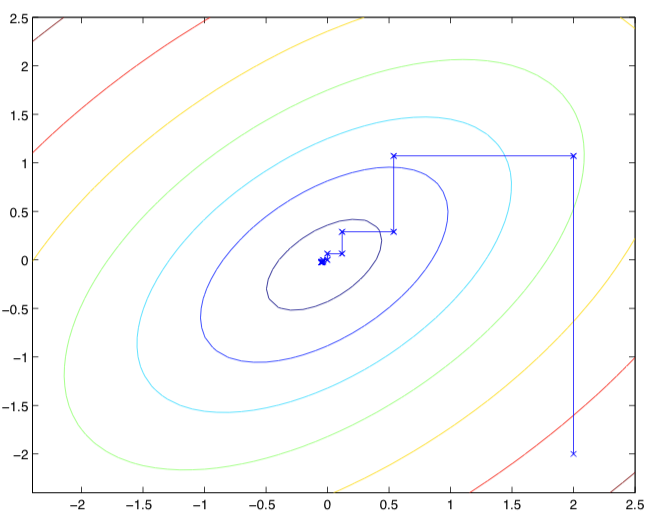
\includegraphics[width=4.4cm]{coorddescent.png}
        \end{center}
        
        \item Coordinate descent can be used to solve lasso regression, as it turns out there is a closed-form solution for $w_i$ (keeping all other features fixed). In practice, it is also commonly used to solve the dual SVM problem.
        
    \end{enumerate}    
    
    \subsection{Decision Trees}
    \begin{enumerate}[label=(\alph*)]
        \item A decision tree is a flowchart-like structure in which each internal node represents a     ``test" on a feature, each branch represents the outcome of the test, and each leaf node represents a class label.
        
        \item Decision tree learning is the problem of learning a sequence of decision rules from data. The rules are typically formulated as ``is feature $x_i > v$?"
        \begin{center}
            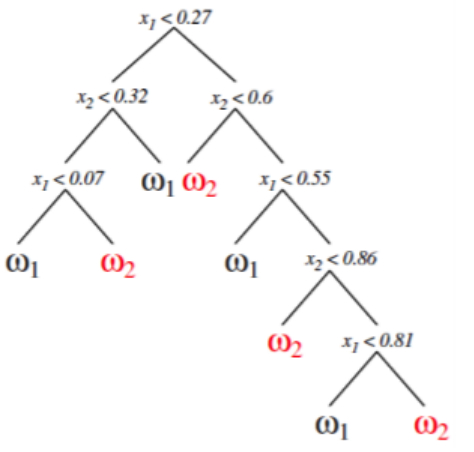
\includegraphics[width=4cm]{dt.png}
        \end{center}
        Decision tree classifiers are often outperformed by more modern classifiers, but are still in use due to their interpretability. Also, combining many decision trees (ensembling) can work well in practice.
        \item Building a decision tree works by repeatedly picking a split-feature, split-value pair. One way to choose splits is inspired by information theory.
        \item The numerical \textit{surprise} of observing that a random variable $X$ takes on value $k$ is $-\log{P(X=k)}$. The \textit{entropy} of $X$, $H(X)$, is defined as
        \begin{align*}
            H(X) &= \mathbb{E}[\text{surprise}] \\
            &= - \sum_k P(X=k) \log{P(X=k)}
        \end{align*}
        It represents the information content of $X$, and is higher when the distribution of its outcomes is closer to uniform rather than biased to one outcome.
        
        \item We want to split on the feature most useful for discriminating between the classes to be learned. This can be done with \textit{information gain}, which, for a particular feature, is the difference between the entropy of the parent and the (weighted) average entropy of its children given a split on that feature. The best split is the one with the highest information gain.
       
        \item For continuous-valued features, we perform the information-gain calculation over a range of threshold values for each feature.
        
        \item For example, say we have $n$ data points $(x_i, y_i)$ where $y_i$ is a class label at some node in the tree. We calculate the entropy of the parent by taking $P(X = y_i) = \frac{\text{count}(y_i)}{n}$. Then, for a particular split, e.g., age $<$ 20, we perform the split and calculate the entropy of the two resulting child nodes similarly.
        
        \item Without a limit on the tree's depth, the classifier can perfectly (overfit) the training set provided no two training points of different classes coincide. Methods of preventing overfitting include imposing depth limits, information gain thresholds, and pruning.
        
        \item \textit{Ensemble methods} involve constructing multiple decision trees to avoid overfitting. In \textit{bagging}, multiple decision trees are constructed by repeatedly resampling training data with replacement, and voting the trees for a consensus prediction.
        
        \item \textit{Random forests}, in addition to bagging, use a modified learning algorithm that selects, at each candidate split in the learning process, a random subset of the features. This helps ensure the decision trees remain diverse and uncorrelated. The size of the random subsample of training points and the number of features per tree are hyperparameters.
        
        \item In \textit{boosting}, which generalizes beyond decision trees, we give weights to each of the simple classifiers (e.g. trees in a random forest). AdaBoost (Adaptive Boosting) is a typical example; it is adaptive in that it incrementally builds an ensemble by training each new classifier to emphasize instances previously mislabeled. In the binary case, the algorithm is:
        \begin{enumerate}[1.]
            \item Initialize weights of training samples: $w_i = \frac{1}{n}$.
            \item For $m=1$ to $M$:
            \begin{enumerate}[i.]
                \item Build a classifier $G_m$ on training set \textit{with replacement} according to probabilities $w_i$.
                \item Compute the weighted error $$e_m = \frac{\sum_i \text{mislabeled } w_i}{\sum_i w_i}$$
                \item Set weight of classifier as $$\alpha_m = \frac{1}{2} \ln \left( \frac{1-e_m}{e_m} \right)$$                
                \item Re-weight training points (then normalize)
                $$
                w_i = w_i \cdot 
                \begin{cases}
                \sqrt{\frac{1 - e_m}{e_m}} \text{ if mislabeled} \\
                \sqrt{\frac{e_m}{1 - e_m}} \text{ otherwise} \\
                \end{cases}
                $$
            \end{enumerate}
        \end{enumerate}
    \end{enumerate}  
    
    \subsection{Convolutional Neural Networks}
    \begin{enumerate}[label=(\alph*)]
        \item Convolutional neural networks (CNNs) are deep, feed-forward artificial neural networks with special layer types (namely convolution and pooling).
        \vspace{-0.4cm}
        \begin{center}
            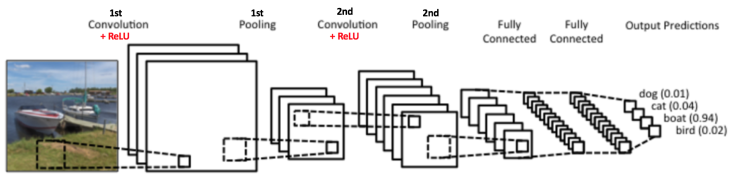
\includegraphics[width=8cm]{convnet.png}
        \end{center}    
        
        \item The first new idea is that of the \textit{convolutional layer}. The layer's parameters consist of a set of learnable filters (or kernels). Each layer of the output volume is an activation map formed by \textit{convolving a kernel} about the input. Convolving means sliding the kernel across the pixels of the previous layer and computing the sum of the elementwise products.
        \begin{center}
            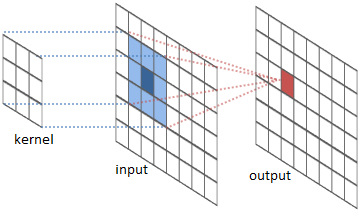
\includegraphics[width=4cm]{conv.png}
        \end{center}
        \vspace{-0.2cm}
        The kernels have a small receptive field, but always extend through the full depth of the input volume. For example, if the input volume is $(w \times h \times d)$, the kernel would be $(k \times k \times d)$, where $k$ is usually small. The $d$ resulting matrices are then combined to form a $(w \times h \times 1)$ activation map. Stacking the activation maps for all filters forms the full output volume of the convolution layer.
        
        \item Kernels act as feature detectors from the original input image. For example, in the table below, we see the effects of convolution of with different filters. \\
        
        
        \begin{tabular}{ccc}
        Operation & Kernel & Result \\
        \midrule
        Identity & $\begin{bmatrix} 0 & 0 & 0 \\ 0 & 1 & 0 \\ 0 & 0 & 0 \end{bmatrix}$ & \adjustimage{height=1.4cm,valign=m}{id.png} \\
        Edge Detection & $\begin{bmatrix} -1 & -1 & -1 \\ -1 & \ \ 8 & -1 \\ -1 & -1 & -1 \end{bmatrix}$ & \adjustimage{height=1.4cm,valign=m}{edge.png} \\
        Sharpen & $\begin{bmatrix} \ \ 0 & -1 & \ \ 0 \\ -1 & \ \ 5 & -1 \\ \ \ 0 & -1 & \ \ 0 \end{bmatrix}$ & \adjustimage{height=1.4cm,valign=m}{sharpen.png} \\
        Gaussian blur & $\frac{1}{16} \begin{bmatrix} 1 & 2 & 1 \\ 2 & 4 & 2 \\ 1 & 2 & 1 \end{bmatrix}$ & \adjustimage{height=1.4cm,valign=m}{gaussianblur.png} \\
        \end{tabular}        
        \item There are two important properties of convolution:
        \begin{enumerate}[1.]
            \item Parameter sharing: the filter values are shared among all the pixels of the input.
            % The result of this convolution is an activation map, and the set of activation maps for each different filter are stacked together along the depth dimension to produce the output volume. 
            \item Local connectivity: each neuron is (spatially) connected to only a small region of the input volume.
        \end{enumerate}
        Both of these properties dramatically reduce the number of parameters from say, a fully connected layer. 
        
        \item In practice, three parameters control the size of the output volume:
        \begin{enumerate}[1.]
            \item Depth: the number of kernels used for the convolution operation, whose outputs are stacked to form the output depth.
            \item Stride: the number of pixels by which we slide the kernels over the input volume. A larger stride means the receptive fields overlap less and the resulting output volume has smaller spatial dimensions. 
            \item Zero-padding: padding the input volume with zeros around the borders so that we can apply the kernel to edge entries. It preserves the spatial size of the input.
        \end{enumerate}
        
        \item Multiple convolutional layers increase the effective receptive field of each neuron. That is, as we go downstream, the value of any single unit is informed by an increasingly large patch of the original image.
        
        \item The next new idea is that of the \textit{pooling layer}, whose sole purpose is to downsample the input. Max pooling is the most common approach: it partitions the input into a set of non-overlapping rectangles and, for each such sub-region, outputs the maximum. It provides a form of translation invariance, because the exact location of a feature is less important than its rough location relative to other features.
        
        It reduces the spatial size (but not depth) of the input, thus reducing computation and reducing overfitting. It is common practice to insert a pooling layer between successive convolutional layers.
        
        \item ReLU is typically applied element-wise to the output of a convolution layer to increase non-linearity without affecting the receptive fields.
        
        \item After several convolutional and max pooling layers, the high-level reasoning in the neural network is done via fully connected layers. A final softmax layer is typically used for classification purposes.
        
        \item Deep CNNs have won many computer vision challenges. There are a variety of architectural choices on how convolutions, pooling, nonlinear activations, and full connections can be composed. In recent years, the trend has been increasingly deep networks.
        
        \item There are several methods that attempt to understand what CNNs have learned:
        \begin{itemize}
            \item Direct visualization of filters, activations, and optimal stimuli (only useful for earlier layers).
            \item Reconstruction by deconvolution: isolate an activation and reconstruct the original image based on that activation alone to see its effect.
            \item Activation maximization: generate an image that maximizes the activation of the network.
            \item Saliency maps: find what locations in the image make a neuron fire.
            \item Code inversion: given a feature representation, determine the original image.
            \item Semantic Interpretation: interpret the activations semantically.
        \end{itemize}
    \end{enumerate}
\end{addmargin}

\section{Unsupervised Learning}
\begin{addmargin}[0.8em]{0.5em}
    \subsection{Dimensionality Reduction}
    \begin{enumerate}[label=(\alph*)]
        \item Unsupervised learning is the task of uncovering hidden structure from ``unlabeled" data. Dimensionality reduction is one such unsupervised method.
        
        \item One approach to dimensionality reduction is feature selection, in which we remove features that we deem to be irrelevant based on some criteria. For example, the Lasso performs feature selection through the use of $L_1$ regularization.
        
        \item Another approach to dimensionality reduction is learning \textit{latent features}. This approach seeks to find new features that are transformations of the given features that represent the data well.
        
        \item Recall PCA: if we have a centered (i.e. zero column mean) data matrix $X \in \mathbb{R}^{n \times d}$, the PCA decomposition amounts to finding the SVD $X = U \Sigma V^\top$. Let $U_k, V_k$ denote the first $k$ columns of $U$ and $V$, respectively, and $\Sigma_k$ denote the upper left $k \times k$ part of $\Sigma$. Then $U_k \Sigma_k \in \mathbb{R}^{n \times k}$ represents the first $k$ principal components of the data while the columns of $V_k$ represent the PCA axes. Further multiplying by $V_k^\top$ gives the reconstruction of the original $X$.

        At test time, $V_k^\top x$ projects a new data point $x$ to the $k$-dimensional latent PCA space, and $V_k V_k^\top x$ reconstructs it. 
        
        \item Sometimes, it does not make sense to find orthogonal directions that capture maximum variance, as PCA does. Independent Components Analysis (ICA) instead seeks directions that are statistically independent, which is more suitable for some applications.
        
        \item Nonnegative Matrix Factorization (NMF) decomposes a non-negative data matrix $X \in \mathbb{R}^{n \times d}$ into $X^\top = BH$, where $B$ and $H$ are non-negative. NMF generates factors with significantly reduced dimensions: if $B$ is $d \times p$ and $H$ is $p \times n$, then $p$ can be significantly less than both $d$ and $n$. The $k$th row of $X$ is the sum of the columns of $B$, weighted according to the entries in the $k$th column of $H$. Each column of $B$ can be interpreted as a meaningful feature. It tends to produce sparser features than PCA.
        
        \item We have thus far discussed linear dimensionality reduction methods that factor the data matrix into a latent representation with a dictionary for projecting the data. But they may fail to capture inherent local geometric structures. Attempts to remedy this include kernel PCA and more sophisiticated methods like Isometric Feature Mapping (IsoMap), Laplacian Eigenmaps, t-Distributed Stochastic Neighbour Embedding (tSNE), etc.
    \end{enumerate}
    
    \subsection{Clustering}
    \begin{enumerate}[label=(\alph*)]
        \item The $k$-means algorithm is popular for its simplicity and usefulness in exploratory data analysis. It works as follows:
        \begin{enumerate}[1.]
            \item Initialize $k$ cluster centers randomly.
            \item Assign all data points to their nearest cluster centers.
            \item Re-estimate the $k$ cluster centers.
            \item Repeat until none of the assignments change.
        \end{enumerate}
        \begin{center}
            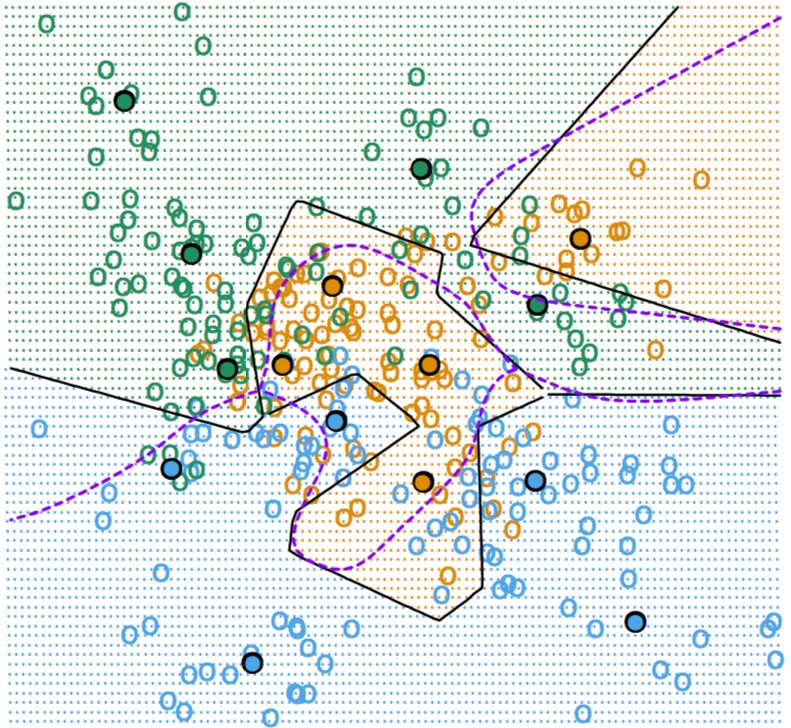
\includegraphics[width=4.6cm]{kmeans.png}
        \end{center}
        Problems with $k$-means include sensitivity to seed choice, difficulty in selecting $k$, and sensitivity to outliers. Formally, it assumes isotropic convex clusters. It is common practice to run $k$-means several times with different initalizations, and pick the clustering that gives the lowest \textit{distortion}, or sum of squared distances between each sample and cluster centroid to which it has been assigned.
    \end{enumerate}  
    
    \subsection{Generative Models}
    \begin{enumerate}[label=(\alph*)]
        \item An \textit{autoencoder} neural network consists of an input layer, an output layer of equal size to the input layer, and one or more hidden layers with limited hidden units connecting them. It attempts to reconstruct its own inputs; that is, it tries to learn an approximation to the identity function, so as to output $\Hat{y}$ that is as close as possible to $y$. They can be used in practice as a form of dimensionality reduction, or to discover interesting structure about the data.
    
        \item Introduced in 2014, \textit{Generative adversarial networks} (GANs) are implemented as a system of two neural networks contesting with each other in a zero-sum game framework. GANs have been used to produce samples of photorealistic images for the purposes of generating new target imagery.
        
        The discriminator network, in the case of images, is a convolutional neural network that assigns a probability that an image is real. The generative network is a kind of convolutional network that uses transpose convolutions, called a deconvolutional network. The idea is to backpropogate the discrimator to find what parts of the image to change in order to yield a greater probability of being real.
    \end{enumerate}     
\end{addmargin}

\pagebreak

\section{Mathematics Appendix}
\begin{addmargin}[0.8em]{0.5em}
\vspace{-0.2cm}
    % A foundation in multivariable calculus, linear algebra, and probability is assumed. The following is a collection of the topics in each field most relevant to machine learning.
    \subsection{Vector Calculus}
    \vspace{-0.2cm}
    \begin{enumerate}[label=(\alph*)]
        \item Optimization is about finding \textbf{extrema}. The set of inputs over which we’re optimizing $\mathcal{X} \subseteq \mathbb{R}^d$ is called the \textit{feasible set}. If $\mathcal{X}$ is the entire domain of the function being optimized, the problem is \textbf{unconstrained}. Otherwise the problem is \textbf{constrained} and may be much harder to solve.
        \item Suppose $f : \mathbb{R}^d \mapsto \mathbb{R}$. A point $x$ is said to be a \textit{local minimum} (resp. \textit{local maximum}) of $f$ in $\mathcal{X}$ if $f(x) \geq f(y)$ (resp. $f(x) \leq f(y)$) for all $y$ in some neighborhood $N \subseteq X$ that contains $x$. 
        \item If $f(x) \leq f(y)$ for all $y \in \mathcal{X}$, then $x$ is a global minimum of $f$ in $\mathcal{X}$ (similarly for global maximum). 
        % \item Observe that maximizing a function $f$ is equivalent to minimizing $-f$, so optimization problems are typically phrased in terms of minimization without loss of generality.
        \item The \textbf{gradient} of $f : \mathbb{R}^d \mapsto \mathbb{R}$, denoted $\nabla f$, is
        \begin{align*}
        \nabla f = 
        \begin{bmatrix} 
        \frac{\partial f}{\partial x_1} \\ \vdots \\ \frac{\partial f}{\partial x_d}
        \end{bmatrix}
        \end{align*}
        We have that $-\nabla f$ points in the direction of steepest descent from $x$.
        \item The \textbf{Jacobian} of $f: \mathbb{R}^n \mapsto \mathbb{R}^m$ is the matrix of first-order partial derivatives:
        \begin{align*}
        \mathbf{J}_f = 
        \begin{bmatrix}
        \frac{\partial f_1}{\partial x_1} & \hdots & \frac{\partial f_1}{\partial x_1} \\
        \vdots & \ddots & \vdots \\
        \frac{\partial f_m}{\partial x_1} & \hdots & \frac{\partial f_m}{\partial x_n}
        \end{bmatrix}
        \end{align*}
        Note that if $m=1$, $\nabla f = \mathbf{J}_f^\top$.
        \item The \textbf{Hessian} matrix $f: \mathbb{R}^d \mapsto \mathbb{R}$ is the matrix of second-order partial derivatives.
        \begin{align*}
        \nabla^2 f =
        \begin{bmatrix}
        \frac{\partial^2 f}{\partial x_1^2} & \hdots & \frac{\partial^2 f}{\partial x_1 \partial x_d} \\
        \vdots & \ddots & \vdots \\
        \frac{\partial^2 f}{\partial x_d \partial x_1} & \hdots & \frac{\partial^2 f}{\partial x_d^2}
        \end{bmatrix}
        \end{align*}
    
    	\item A function $f$ is convex if $$\lambda f(x_1) + (1 - \lambda) f(x_2) \geq f(\lambda x_1 + (1-\lambda) x_2)$$ for any $x_1$ and $x_2$ in the domain of $f$ and $0 \leq \lambda \leq 1$.
    	
    	\item Equivalently, a function $f$ is convex if its Hessian matrix is positive semi-definite everywhere on the domain of $f$. 
        
        \item A \textit{convex set} is a set $S$ where $$x_1 \in S, x_2 \in S \implies \lambda x_1 + (1 - \lambda) x_2 \in S,$$ where $0 \leq \lambda \leq 1$. In words, if $x_1$ and $x_2$ are in $S$, then everything ``in between'' $x_1$ and $x_2$ is also in $S$.
        
        \item The \textit{convex hull} of a set $S$ of points in Euclidean space is the smallest convex set that contains $S$. 
        
    	\item A function $f$ is convex if the set $S_f = \{(x, y) \mid x \in \mathbb{R}^n, y \in \mathbb{R}, y \geq f(x)\}$ is convex. The set $S_f$ is called the \emph{epigraph} of the function $f$. It is all the points that lie ``above'' the curve $f$.
    	
    	\item Convexity is useful for the following reason: if $f$ is convex in $\mathcal{X}$, then any local minimum of $f$ in $\mathcal{X}$ is also a global minimum.    	
        
        \item For the OLS loss function $f(x) = \|Ax-y\|_2^2$,
        % \begin{align*}
        % f(x) &= \|Ax-y\|^2 \\
        % &= (Ax-y)^\top(Ax-y) \\
        % &= y^\top y - 2x^\top A y + x^\top A^\top A x
        % \end{align*}
        % So that
        \begin{align*}
        \frac{\partial f}{\partial x} = -2A^\top y + 2 A^\top A x
        \end{align*}
        so that the Hessian is then
        \begin{align*}
        \frac{\partial^2 f}{\partial x \partial x^\top} = 2 A^\top A
        \end{align*}
        which is positive semi-definite.
        
        \item If $f$ and $g$ are convex, then
        \begin{itemize}
        \item $\alpha f + \beta g$ for $\alpha, \beta \geq 0$ is convex
        \item $\max(f,g)$ is convex
        \end{itemize}
        
        \item Let $A$ be a matrix and $x, w$ be vectors. Common gradients include:
        \begin{itemize}
        \item $\nabla_{x} ( w^\top x ) = w$
        \item $\nabla_{x} ( x^\top x ) = 2x$
        \item $\nabla_{x} ( x ) = I$
        \item $\nabla_{x} ( Ax ) = A^\top $
        \item $\nabla_{x} ( x^\top A ) = A$
        \item $\nabla_{x} ( x^\top Ax ) = (A + A^\top)x$
        \item $\nabla_{A} ( x^\top Ax ) = \frac{\partial}{\partial A} \text{tr}(x x^\top A) = (x x^\top)^\top = x x^\top$
        \end{itemize}
    \end{enumerate}
    \vspace{-0.9cm}
    \subsection{Linear Algebra}
    \vspace{-0.3cm}
    \begin{enumerate}[label=(\alph*)]
        \item An \textbf{orthogonal} matrix $A$ is such that $A^{-1} = A^\top$. They preserve 2-norms: $\| Ax \|_2 = \| x \|_2$.
        
        \item A \textbf{symmetric} matrix $A$ is such that $A=A^\top$. They have a convenient spectral decomposition: $A = Q \Lambda Q^\top$ where $Q$ consists of an orthonormal basis of $\mathbb{R}^n$ of eigenvectors of $A$ and $\Lambda = \text{diag}(\lambda_1, \hdots, \lambda_n)$.
        
        \item A symmetric matrix $A$ is called \textbf{positive semi-definite} if for all vectors $x^\top A x \geq 0$. This is equivalent to having all nonnegative eigenvalues. If the inequality is strict, $A$ is called \textbf{positive definite}.
        
        \item A positive semi-definite matrix $A$ has a unique square root $A^{1/2}$ that is also positive semi-definite.
        
        % \item \textbf{Negative definite} and \textbf{negative semi-definite matrices} are defined similarly, and a symmetric matrix is \textbf{indefinite} if it is neither positive semi-definite nor negative semi-definite.
        \item Let $A \in \mathbb{R}^{m \times n}$. Then $A^\top A$ is symmetric and thus orthogonally diagonalizable. Let $\{ v_1, \hdots, v_n \}$ be an orthonormal basis for $\mathbb{R}^n$ consisting of eigenvectors of $A^\top A$, and $\lambda_1, \hdots, \lambda_n$ be the associated eigenvalues. For $1 \leq i \leq n$,
        \begin{align*}
            \| Av_i \|^2 = (Av_i)^\top Av_i = v_i^\top A^\top A v_i = v_i^\top (\lambda_i v_i) = \lambda_i
        \end{align*}
        The eigenvalues of $A^\top A$ are nonnegative, so $A^\top A$ is positive semi-definite. The \textbf{singular values} of $A$, denoted $\sigma_1, \hdots, \sigma_n$,  are the square roots of the eigenvalues of $A^\top A$ arranged in decreasing order.
        
        \item Let $A \in \mathbb{R}^{m \times n}(\mathbb{R})$ with singular values $\sigma_1 \geq \sigma_2 \geq \hdots \geq \sigma_n$. The \textbf{singular value decomposition} of $A$ is given by 
        $$
        A = U \Sigma V^\top 
        $$
        where $U \in \mathbb{R}^{m \times m}$ and $V \in \mathbb{R}^{n \times n}$ are orthogonal matrices and $\Sigma=\text{diag}(\sigma_1, \hdots, \sigma_n)$.
        \item The columns of $U$ are called the left-singular vectors of $A$, and are unit eigenvectors of $AA^\top$. The columns of $V$ are called the right-singular vectors of $A$, and are unit eigenvectors of $A^\top A$.
        \item Let $A \in \mathbb{R}^{m \times n}$ with rank $r$ and SVD $A=U\Sigma V^\top$. Let $\Sigma^\dagger$ be the $n \times m$ matrix defined by
        \begin{align*}
            \Sigma_{ij}^\dagger = 
                \left\{
                \begin{array}{ll}
                  \frac{1}{\sigma_i} \text{ if $i=j \leq r$} \\
                  0 \text{ otherwise}
                \end{array}
                \right.
        \end{align*}
        Then $A^\dagger = V \Sigma^\dagger U^\top$. $A^\dagger$ is called the \textbf{pseudoinverse} of $A$.

        \item The \textbf{norm} of $x \in \mathbb{R}^n$ is $\| x \| = \sqrt{ \langle x,x \rangle }$. For all $x,y \in \mathbb{R}^n$, the following hold:
        \begin{enumerate}
            \item $\| cx \| = |c| \cdot \| x \|$
            \item $\| x \| \geq 0$ with equality iff $x=\vec{0}$
            \item $\| x + y \| \leq \| x \| + \| y \|$ (triangle inequality)
        \end{enumerate}
        
        \item Some specific norms on $\mathbb{R}^n$ include
        \begin{align*}
            &\| x \|_1 = \sum_{i=1}^n | x_i | \\
            &\| x \|_2 = \sqrt{\sum_{i=1}^n  x_i^2 } \\
            &\| x \|_p = \left( \sum_{i=1}^n  |x_i|^p  \right)^\frac{1}{p} \\
            &\| x \|_\infty = \max_{1 \leq i \leq n} |x_i|
        \end{align*}
        
        \item The standard inner product on $\mathbb{R}^n$ is given by
        $$
        \langle x, y \rangle = x^\top y
        $$
        
        \item The \textbf{trace} of a square matrix is the sum of its diagonal entries.
        \begin{itemize}
        \item $\text{tr}(A + B) = \text{tr}(A) + \text{tr}(B)$
        \item $\text{tr}(\alpha A) = \alpha \text{tr}(A)$
        \item $\text{tr}(ABC) = \text{tr}(BCA) = \text{tr}(CAB)$
        \end{itemize}
        
        \item The \textbf{Frobenius norm} for a matrix $A \in \mathbb{R}^{m \times n}$ is given by $$\| A \|_F = \sqrt{\text{tr}(A^\top A)} = \sqrt{\sum_{i=1}^{m} \sum_{j=1}^{n} |A_{ij}|^2}$$
        
        \item The scalar $x^\top A x$ for a symmetric matrix $A$ is called a \textbf{quadratic form}. The isocontours of $f(x) = x^\top Ax$ are ellipsoids such that the axes point in the directions of the eigenvectors of $A$, and the radii of these axes are proportional to the inverse square roots of the corresponding eigenvalues.
        
        \item The \textbf{Rayleigh quotient} for a symmetric matrix $A$ is defined by 
        $$
        R_A(x) = \frac{x^\top A x}{x^\top x}
        $$
        For any $x$ such that $\| x \|_2=1$, 
        $$
        \lambda_{\text{min}}(A) \leq x^\top A x \leq \lambda_{\text{max}}(A)
        $$
        with equality iff $x$ is a corresponding eigenvector. Consequently, for any $x \neq \vec{0}$,
        $$
        \lambda_{\text{min}}(A) \leq R_A(x) \leq \lambda_{\text{max}}(A)
        $$
    \end{enumerate}
    \vspace{-0.2cm}
    \subsection{Probability}
    \vspace{-0.2cm}
    \begin{enumerate}[label=(\alph*)]
    \item Bayes' Rule: If $A$ and $B$ are events, then
    $$
    P(A | B) = \frac{P(B|A)P(A)}{P(B)}
    $$
    It is sometimes useful to omit the normalizing constant and write
    $$
    P(A|B) \propto P(A)P(B|A)
    $$
    $P(A)$ is often referred to as the \textit{prior}, $P(A|B)$ as the \textit{posterior}, and $P(B|A)$ as the \textit{likelihood}.
    
    \item If $\{ A_i \}_{i=1}^{n}$ is a set of events, disjoint or not, then
    $$
    P \left( \bigcup_i A_i) \right) \leq \sum_{i} P(A_i)
    $$
    This inequality is called the \textbf{union bound}.
    
    \item The \textbf{variance} of a random variable $X$ is given by
    $$
    \text{Var}(X) = \mathbb{E}[X^2] - \mathbb{E}[X]^2
    $$
    We have
    $$
    \text{Var}(\alpha X + \beta) = \alpha^2 \text{Var}(X)
    $$
    \item \textbf{Covariance} is a measure of the linear relationship between two random variables.
    \begin{align*}
    \text{Cov}(X,Y) = \mathbb{E}[XY] - \mathbb{E}[X] \mathbb{E}[Y]
    \end{align*}
    We have
    \begin{itemize}
    \item $\text{Cov}(\alpha X + \beta Y, Z) = \alpha \text{Cov}(X, Z) + \beta \text{Cov}(Y, Z)$
    \item $\text{Cov}(X, \alpha Y + \beta Z) = \alpha \text{Cov}(X, Y) + \beta \text{Cov}(X, Z)$
    \end{itemize}
    
    \item Normalizing the covariance gives the \textbf{Pearson correlation coefficient}:
    \begin{align*}
    \rho(X, Y) = \frac{\text{Cov}(X,Y)}{\sqrt{\text{Var(X)\text{Var(Y)}}}}
    \end{align*}
    Correlation also measures the linear relationship between two variables, but unlike covariance always lies between $1$ and $-1$. Two variables are said to be uncorrelated if $\text{Cov}(X, Y) = 0$. If two variables are independent, then they are uncorrelated, but the converse does not hold in general. Note that $\rho(aX + b, cY + d) = \rho(X,Y)$, i.e. it is invariant to affine transformations.
    
    \item Multivariate distributions which give distributions of \textbf{random vectors}:
    $$
    \mathbf{X} = \begin{bmatrix} X_1 \\ \vdots \\ X_n \end{bmatrix} 
    $$
    Expectation of a random vector is expectation applied component-wise. The variance is generalized by the covariance matrix $\Sigma$:
    \begin{align*}
    \Sigma &= \mathbb{E}[(\mathbf{X} - \mathbb{E}[\mathbf{X}])(\mathbf{X} - \mathbb{E}[\mathbf{X}])^\top]
    \end{align*}
    Expliclitly, 
    \begin{align*}
    \Sigma = 
    \begin{bmatrix}
    \text{Var}(X_1) & \text{Cov}(X_1, X_2) & \hdots & \text{Cov}(X_1, X_n) \\
    \text{Cov}(X_2, X_1) & \text{Var}(X_2) & \hdots & \text{Cov}(X_2, X_n) \\
    \vdots & \vdots & \ddots & \vdots \\
    \text{Cov}(X_n, X_1) & \text{Cov}(X_n, X_2) & \hdots & \text{Var}(X_n)
    \end{bmatrix}
    \end{align*}
    Note that $\Sigma$ is positive semi-definite.
    
    \item The \textbf{cross-covariance} matrix of random vectors $\mathbf{X}$ and $\mathbf{Y}$ is given by
    $$
    \Sigma_{XY} = \mathbb{E}[(\mathbf{X} - \mathbb{E}[\mathbf{X}])(\mathbf{Y} - \mathbb{E}[\mathbf{Y}])^\top]
    $$
    
    \item The multivariate \textbf{Gaussian distribution}, also known as the normal distribution, is a continuous distribution parameterized by its mean $\mu \in \mathbb{R}^d$ and covariance matrix $\Sigma \in \mathbb{R}^{d \times d}$, with PDF
    \begin{align*}
    P(x) = \frac{1}{\sqrt{(2\pi)^d \det{\Sigma}}} \exp \left( -\frac{1}{2} (x-\mu)^\top \Sigma^{-1} (x-\mu) \right)
    \end{align*}
    We write $\mathbf{X} \sim \mathcal{N}(\mu, \Sigma)$ to denote that $\mathbf{X}$ is normally distributed with mean $\mu$ and variance $\Sigma$.
    
    Given $n$ i.i.d. samples $x_1, \ldots, x_n \in \mathbb{R}^d$ from $\mathbf{X} \sim \mathcal{N}(\mu, \Sigma)$, the log-likelihood is given by
    $$
    -\frac{n}{2} \log{|\Sigma|} -\frac{1}{2} \sum_{i=1}^{n} (x_i - \mu)^\top \Sigma^{-1} (x_i - \mu) + \text{constant}
    $$
    From this we derive the MLEs of $\mu$ and $\Sigma$:
    \begin{align*}
    \hat{\mu} &= \frac{1}{n} \sum_{i=1}^{n} x_i \hspace{8pt}, \hat{\Sigma} = \frac{1}{n} \sum_{i=1}^{n} (x_i - \hat{\mu}) (x_i - \hat{\mu})^\top
    \end{align*}
    
    \item A probabalistic approach to parameter estimation is \textbf{maximum likelihood estimation (MLE)}. The basic principle of MLE is to choose values that ``explain" the data best by maximizing the probability of the observed data seen as a function of the parameters $\theta$. That is,
    $$
    \hat{\theta}_{\text{MLE}} = \arg\max_{\theta} \mathcal{L}(\theta)
    $$
    where $\mathcal{L}$ is the likelihood function
    $$
    \mathcal{L}(\theta) = P(x_1, \hdots, x_n; \theta)
    $$
    If we assume the observations are i.i.d., then 
    $$
    P(x_1, \hdots, x_n; \theta) = \prod_{i=1}^n P(x_i;\theta)
    $$
    We can take the log to get the log-likelihood:
    $$
    \log{\mathcal{L}(\theta)} = \sum_{i=1}^{n} \log{P(x_i; \theta)}
    $$
    Since log is a monotonically increasing function, any maximizer of $\log{\mathcal{L}}$ also maximizes $\mathcal{L}$.
    
    \item A Bayesian way to fit parameters is through \textbf{maximum a posteriori estimation (MAP)}. In this approach, the parameters are assumed to be random variables with a specified prior distribution $P(\theta)$. Through Bayes' rule and ignoring the normalizing constant, we have
    $$
    \hat{\theta}_{\text{MAP}} = \arg\max_{\theta} P(\theta)P(x_1, \hdots, x_n | \theta)
    $$
    If we assume the observations are i.i.d., then we take the log to get
    $$
    \hat{\theta}_{\text{MAP}} = \arg\max_{\theta} \left( \log{P(\theta)} + \sum_{i=1}^n \log{P(x_i | \theta)} \right)
    $$    
    \end{enumerate}
\end{addmargin}

\end{multicols}
\end{document}